% ==============================================================================
% INTEGRATED AGRICULTURAL DATA SYSTEM - FINAL YEAR PROJECT THESIS
% Addis Ababa Science and Technology University
% Single self-contained .tex file — ~19,000 words, ~60 pages
% Compile: pdflatex iads-thesis && bibtex iads-thesis && pdflatex iads-thesis && pdflatex iads-thesis
% ==============================================================================

\documentclass[12pt,a4paper,oneside]{report}

% ── Packages ──────────────────────────────────────────────────────────────────
\usepackage[utf8]{inputenc}
\usepackage[T1]{fontenc}
\usepackage{amsmath,amssymb}
\usepackage{graphicx}
\usepackage{hyperref}
\usepackage{geometry}
\usepackage{setspace}
\usepackage{tocloft}
\usepackage{booktabs}
\usepackage{tabularx}
\usepackage{longtable}
\usepackage{enumitem}
\usepackage{caption}
\usepackage{float}
\usepackage{xcolor}
\usepackage{listings}
\usepackage[numbers,sort&compress]{natbib}
\usepackage{appendix}
\usepackage{fancyhdr}
\usepackage{titlesec}
\usepackage{array}
\usepackage{multirow}
\usepackage{makecell}
\usepackage{tikz}
\usetikzlibrary{shapes.geometric, arrows, positioning, fit, backgrounds, calc, shadows}
\usepackage{pgfplots}
\pgfplotsset{compat=1.18}

% ── TikZ styles ───────────────────────────────────────────────────────────────
\tikzstyle{startstop} = [rectangle, rounded corners, minimum width=3cm, minimum height=0.9cm, text centered, draw=black!60, fill=red!15]
\tikzstyle{process} = [rectangle, minimum width=3cm, minimum height=0.9cm, text centered, draw=black!60, fill=blue!10]
\tikzstyle{decision} = [diamond, minimum width=2.6cm, minimum height=0.9cm, text centered, draw=black!60, fill=green!10]
\tikzstyle{storage} = [trapezium, trapezium left angle=70, trapezium right angle=110, minimum width=2.6cm, minimum height=0.9cm, text centered, draw=black!60, fill=orange!10]
\tikzstyle{arrow} = [thick,->,>=stealth]
\tikzstyle{cloud} = [ellipse, minimum width=2.6cm, minimum height=0.9cm, text centered, draw=black!60, fill=yellow!15]

% ── Embed references ──────────────────────────────────────────────────────────
\usepackage{filecontents}
\begin{filecontents}[overwrite]{\jobname.bib}
@techreport{fao2023,
  author = {{FAO}},
  title  = {Leveraging Automation for Agriculture Transformation},
  institution = {Food and Agriculture Organization of the United Nations},
  address = {Rome}, year = {2023}}
@inproceedings{islam2021,
  author = {M. D. Islam and S. Ahmed and R. Karim},
  title = {Design of Offline-First Mobile Apps for Rural Areas},
  booktitle = {Proc.\ IEEE Global Humanitarian Technology Conference},
  address = {Seattle, WA, USA}, year = {2021}, pages = {112--119}}
@article{trivedi2021,
  author = {N. K. Trivedi and V. Gautam and A. Anand and H. M. Aljahdali and S. G. Villar and D. Anand and N. Goyal and S. Kadry},
  title = {Early detection and classification of tomato leaf disease using high-performance deep neural network},
  journal = {Sensors}, volume = {21}, number = {23}, pages = {7987}, year = {2021}}
@article{anderson2020,
  author = {J. A. Anderson},
  title = {Human-Centered System Design for Development},
  journal = {ACM Transactions on Computer-Human Interaction},
  volume = {27}, number = {4}, pages = {1--32}, year = {2020}}
@techreport{worldbank2022,
  author = {{World Bank}},
  title = {Ethiopia's Digital Economy: A New Frontier},
  institution = {World Bank Group}, address = {Washington, D.C.}, year = {2022}}
@article{ahmed2021,
  author = {S. Ahmed and M. B. Hasan and T. Ahmed and R. K. Sony and M. H. Kabir},
  title = {Less is More: Lighter and Faster Deep Neural Architecture for Tomato Leaf Disease Classification},
  journal = {arXiv preprint arXiv:2109.02394}, year = {2021}}
@article{efficientnet2023,
  author = {{Anonymous}},
  title = {A Smartphone-Based Detection System for Tomato Leaf Disease Using EfficientNetV2B2},
  journal = {Sensors}, volume = {23}, number = {21}, pages = {8685}, year = {2023}}
@article{sharma2023,
  author = {A. Sharma and P. Kumar and R. Singh},
  title = {Deep learning based ensemble model for accurate tomato leaf disease classification},
  journal = {Computers and Electronics in Agriculture},
  volume = {202}, pages = {107385}, year = {2023}}
@inproceedings{lewis2020,
  author = {P. Lewis and E. Perez and A. Piktus and F. Petroni and V. Karpukhin and N. Goyal and H. K\"{u}ttler and M. Lewis and W. Yih and T. Rockt\"{a}schel and S. Riedel and D. Kiela},
  title = {Retrieval-Augmented Generation for Knowledge-Intensive NLP Tasks},
  booktitle = {Advances in Neural Information Processing Systems}, year = {2020}, pages = {9459--9474}}
@misc{scikit2024,
  author = {{scikit-learn}},
  title = {Gradient Boosting Regressor Documentation}, year = {2024},
  howpublished = {\url{https://scikit-learn.org/stable/modules/generated/sklearn.ensemble.GradientBoostingRegressor.html}}}
@misc{anthropic2025,
  author = {{Anthropic}},
  title = {Claude Haiku Model Documentation}, year = {2025},
  howpublished = {\url{https://docs.anthropic.com/en/docs/about-claude/models}}}
@techreport{digitalethiopia2025,
  author = {{Government of Ethiopia}},
  title = {Digital Ethiopia 2025: A Digital Strategy for Ethiopia},
  address = {Addis Ababa, Ethiopia}, year = {2020}}
@article{davis1989,
  author = {F. D. Davis},
  title = {Perceived Usefulness, Perceived Ease of Use, and User Acceptance of Information Technology},
  journal = {MIS Quarterly}, volume = {13}, number = {3}, pages = {319--340}, year = {1989}}
@article{vanklinken2022,
  author = {R. van Klinken and S. M. E. Farrow and T. J. V. Higgins},
  title = {Agricultural data systems in sub-Saharan Africa: A review},
  journal = {Agricultural Systems}, volume = {196}, pages = {103337}, year = {2022}}
@inproceedings{patel2020,
  author = {S. Patel and S. K. Patel and A. K. Verma},
  title = {A comparative study of gradient boosting algorithms for crop yield prediction},
  booktitle = {Proc.\ International Conference on Computing, Communication and Networking Technologies},
  year = {2020}, pages = {1--6}}
@article{zhang2018,
  author = {Y. Zhang and A. E. R. M. Z. Arefin and N. K. H. Al-Mamun},
  title = {A review of deep learning techniques for crop yield prediction},
  journal = {Computers and Electronics in Agriculture},
  volume = {153}, pages = {320--331}, year = {2018}}
@article{shahhosseini2021,
  author = {M. Shahhosseini and R. A. Martinez-Feria and G. Hu and S. V. Archontoulis},
  title = {Maize yield and nitrate loss prediction with machine learning algorithms},
  journal = {Environmental Research Letters},
  volume = {16}, number = {2}, pages = {024026}, year = {2021}}
@misc{nextjs2025,
  author = {{Vercel}},
  title = {Next.js Documentation}, year = {2025},
  howpublished = {\url{https://nextjs.org/docs}}}
@misc{adonisjs2025,
  author = {{AdonisJS}},
  title = {AdonisJS Documentation}, year = {2025},
  howpublished = {\url{https://docs.adonisjs.com}}}
@misc{fastapi2025,
  author = {{FastAPI}},
  title = {FastAPI Documentation}, year = {2025},
  howpublished = {\url{https://fastapi.tiangolo.com}}}
@misc{openmrs2023,
  author = {{OpenMRS}},
  title = {OpenMRS: Open Medical Record System}, year = {2023},
  howpublished = {\url{https://openmrs.org}}}
@misc{dhis22023,
  author = {{DHIS2}},
  title = {DHIS2: District Health Information System}, year = {2023},
  howpublished = {\url{https://dhis2.org}}}
@article{naik2024,
  author = {A. Naik and B. K. Patel and C. R. Sharma},
  title = {RAG-based question answering over structured databases: A survey},
  journal = {arXiv preprint arXiv:2403.09385}, year = {2024}}
\end{filecontents}

% ── Page geometry ─────────────────────────────────────────────────────────────
\geometry{margin=1in}
\onehalfspacing

% ── Header / Footer ───────────────────────────────────────────────────────────
\pagestyle{fancy}
\fancyhf{}
\fancyhead[R]{\thepage}
\fancyhead[L]{\leftmark}
\renewcommand{\headrulewidth}{0.4pt}

% ── Chapter formatting ────────────────────────────────────────────────────────
\titleformat{\chapter}[display]
  {\normalfont\bfseries\Large\centering}
  {\chaptertitlename\ \thechapter}{12pt}{}
\titlespacing*{\chapter}{0pt}{-20pt}{20pt}

% ── Code listings ─────────────────────────────────────────────────────────────
\lstset{
  basicstyle=\ttfamily\small,
  breaklines=true,
  frame=single,
  numbers=left,
  numberstyle=\tiny,
  xleftmargin=2em,
  language=Python,
  captionpos=b,
}

\newcommand{\term}[1]{\textit{#1}}
\newcommand{\code}[1]{\texttt{#1}}
\newcolumntype{L}[1]{>{\raggedright\arraybackslash}p{#1}}
\newcolumntype{C}[1]{>{\centering\arraybackslash}p{#1}}

\begin{document}

% ==============================================================================
% TITLE PAGE
% ==============================================================================
\begin{titlepage}
\begin{center}
\vspace*{2cm}
{\LARGE\bfseries ADDIS ABABA SCIENCE AND TECHNOLOGY UNIVERSITY}\\[0.5cm]
{\large College of Engineering}\\[0.2cm]
{\large Department of Electrical and Computer Engineering}\\[1.5cm]
{\Huge\bfseries Integrated Agricultural Data System}\\[1.5cm]
{\large Final Year Project Report}\\[1cm]
\begin{tabular}{ll}
\textbf{Name} & \textbf{ID} \\
Kidan Dibekulu  & ETS0916/14 \\
Kaleab Kebede   & ETS0857/14 \\
Kalkidan Yishak & ETS0888/14 \\
Dagmawi Shewaye & ETS0425/14 \\
\end{tabular}\\[1.5cm]
{\large Submitted to Addis Ababa Science and Technology University}\\
{\large for the award of Bachelor of Science Degree in}\\
{\large Electrical and Computer Engineering (Computer Engineering)}\\[1cm]
{\large Advisor: Ir. Esubalew M.}\\[1cm]
{\large June 2026}
\end{center}
\end{titlepage}

% ==============================================================================
% DECLARATION
% ==============================================================================
\chapter*{Declaration}
\addcontentsline{toc}{chapter}{Declaration}
We, the undersigned, hereby declare that the project work entitled ``Integrated Agricultural Data System'' is our original work and has been carried out in partial fulfillment of the requirements for the Bachelor of Science Degree in Computer Engineering at Addis Ababa Science and Technology University.

This project has not been submitted, in whole or in part, to any other institution or university for the award of any academic degree or diploma. All sources of information used during the course of this research have been duly acknowledged and referenced. Where the work of others has been quoted or paraphrased, the source has been explicitly cited in accordance with standard academic referencing practices.

The results, analyses, and conclusions presented in this report are based on our own implementation, experimentation, and findings, conducted under the supervision of Ir. Esubalew M. The system described in this report has been developed and tested by the undersigned team members, and all code, documentation, and data are the product of our collective effort.

We understand that any violation of academic honesty and integrity may lead to disciplinary action as per the university's regulations.

\vspace{1cm}
\begin{tabular}{lll}
\textbf{Name} & \textbf{ID Number} & \textbf{Signature} \\[0.3cm]
1. Dagmawi Shewaye  & ETS0425/14 & \rule{5cm}{0.4pt} \\[0.3cm]
2. Kaleab Kebede    & ETS0857/14 & \rule{5cm}{0.4pt} \\[0.3cm]
3. Kalkidan Yishak  & ETS0888/14 & \rule{5cm}{0.4pt} \\[0.3cm]
4. Kidan Dibekulu   & ETS0916/14 & \rule{5cm}{0.4pt} \\
\end{tabular}

% ==============================================================================
% ACKNOWLEDGEMENT
% ==============================================================================
\chapter*{Acknowledgement}
\addcontentsline{toc}{chapter}{Acknowledgement}
First and foremost, we would like to express our deepest gratitude to the Almighty God for granting us the strength, perseverance, and wisdom to complete this project successfully.

We are sincerely thankful to our advisor, Mr.\ Esubalew M., for his continuous guidance, insightful feedback, and dedicated support throughout the course of this project. His expertise in software engineering and system architecture greatly shaped the direction and quality of our work. His encouragement during challenging phases of development and his insistence on rigorous technical standards were instrumental in achieving the outcomes presented in this report.

We would also like to thank the faculty and staff of the Department of Electrical and Computer Engineering, Addis Ababa Science and Technology University, for providing the academic resources, laboratory infrastructure, and supportive learning environment that enabled us to conduct this research. The department's commitment to practical, hands-on engineering education has been invaluable.

Our heartfelt appreciation goes to the creators and maintainers of open-source technologies including AdonisJS, Next.js, FastAPI, scikit-learn, Leaflet.js, Recharts, PostgreSQL, and the many other libraries used in this project. We are particularly grateful to the communities behind these projects for their comprehensive documentation, responsive issue tracking, and continuous improvements.

We extend our thanks to the Ethiopian Agricultural Transformation Institute and the Ministry of Agriculture for their publicly available reports that informed our understanding of the agricultural data landscape in Ethiopia. Their work in advancing digital agriculture provided essential context and motivation for this project.

We are immensely grateful to our families, friends, and peers for their unwavering encouragement, motivation, and moral support during challenging times. Their belief in us has been a constant source of inspiration, and their patience during late nights and long work sessions has been deeply appreciated.

Finally, this work is the result of collective effort, dedication, and shared vision, and we are proud to present it as a contribution to the advancement of digital agriculture and intelligent systems in Ethiopia.

% ==============================================================================
% TABLE OF CONTENTS
% ==============================================================================
\tableofcontents
\newpage

% ==============================================================================
% LIST OF FIGURES
% ==============================================================================
\listoffigures
\newpage

% ==============================================================================
% LIST OF TABLES
% ==============================================================================
\listoftables
\newpage

% ==============================================================================
% ABBREVIATIONS
% ==============================================================================
\chapter*{List of Abbreviations}
\addcontentsline{toc}{chapter}{List of Abbreviations}
\begin{tabular}{ll}
AI     & Artificial Intelligence \\
API    & Application Programming Interface \\
CNN    & Convolutional Neural Network \\
CRUD   & Create, Read, Update, Delete \\
CSV    & Comma-Separated Values \\
FAO    & Food and Agriculture Organization \\
GB     & Gradient Boosting \\
HTTP   & Hypertext Transfer Protocol \\
IADS   & Integrated Agricultural Data System \\
JWT    & JSON Web Token \\
LLM    & Large Language Model \\
MAE    & Mean Absolute Error \\
ML     & Machine Learning \\
MVC    & Model-View-Controller \\
NDVI   & Normalized Difference Vegetation Index \\
NGO    & Non-Governmental Organization \\
ORM    & Object-Relational Mapping \\
RAG    & Retrieval-Augmented Generation \\
RBAC   & Role-Based Access Control \\
RMSE   & Root Mean Square Error \\
REST   & Representational State Transfer \\
SQL    & Structured Query Language \\
TAM    & Technology Acceptance Model \\
UI     & User Interface \\
UUID   & Universally Unique Identifier \\
VPS    & Virtual Private Server \\
XLSX   & Microsoft Excel Open XML Spreadsheet \\
\end{tabular}
\newpage

% ==============================================================================
% ABSTRACT
% ==============================================================================
\chapter*{Abstract}
\addcontentsline{toc}{chapter}{Abstract}
Agricultural data collection and management in Ethiopia face significant challenges due to unreliable internet connectivity, fragmented record-keeping systems, and lack of access to predictive analytics. Traditional methods relying on paper-based surveys are time-consuming, error-prone, and inaccessible in many rural and under-resourced areas. This study presents the development of an Integrated Agricultural Data System (IADS), an offline-capable geospatial crop monitoring platform that combines offline-first architecture, AI-powered analytics, and stakeholder-specific dashboards to address these challenges.

The system integrates five core components: an offline data synchronization module using a queue-and-check mechanism for reliable field data collection in low-connectivity environments; a legacy data import tool for bulk ingestion of CSV and Excel files with automatic schema detection supporting over 80 column header variations; a scikit-learn-based Gradient Boosting Regressor for crop yield prediction achieving a Mean Absolute Error of 863.54~kg/ha and Root Mean Square Error of 1539.96~kg/ha; a Retrieval-Augmented Generation (RAG) system using Anthropic Claude or Cerebras large language models enabling natural language queries on agricultural datasets; and stakeholder-specific dynamic dashboards tailored for government, NGO, trader, and researcher users with role-based access control across seven user roles.

The training dataset consisted of 2,000 crop yield records spanning 2015 to 2024 across six major Ethiopian regions (Afar, Amhara, Oromia, Sidama, SNNPR, Tigray) covering eight crop types (teff, wheat, maize, barley, sorghum, sesame, chickpea, coffee) across two growing seasons (Meher and Belg). The Gradient Boosting model was trained on seven features including area cultivated, rainfall, temperature, fertilizer amount, year, crop type, and season.

Integrated into a full-stack web application built with AdonisJS 7 on the backend and Next.js 16 on the frontend, the system enables field agents to collect and synchronize agricultural data offline, upload historical datasets, and allows stakeholders to query agricultural data using natural language through the RAG interface. The system implements role-based dashboards with interactive maps using Leaflet.js and charts using Recharts, along with comprehensive audit logging and data governance features across 108 RESTful API endpoints and 15 database tables.

This project contributes to the field of digital agriculture by offering a comprehensive, accessible, and accurate platform that empowers stakeholders to make timely decisions, reduce crop losses, and promote sustainable farming practices in connectivity-constrained environments, directly supporting Ethiopia's Digital Ethiopia 2025 strategy.

% ==============================================================================
% CHAPTER 1: INTRODUCTION
% ==============================================================================
\chapter{Introduction}

\section{Background of the Study}
Agricultural data systems refer to the collection of technologies, processes, and methodologies used to capture, store, analyze, and disseminate information related to farming activities, including farmer demographics, crop types, field sizes, yields, and disease occurrences. The significance of these systems lies in their potential to enhance decision-making, ensure food security, and reduce economic losses in agriculture. Traditional methods of data collection rely heavily on paper surveys and manual entry by extension workers, which can be time-consuming, labor-intensive, and prone to human error \cite{vanklinken2022}. As a result, automated and technology-driven solutions have gained increasing attention from researchers, policymakers, and development organizations worldwide.

Agriculture undeniably remains the cornerstone of the Ethiopian economy, providing employment to over 80 percent of the population and contributing approximately 33 percent to the national Gross Domestic Product. The sector is characterized by smallholder farming systems, with the majority of farmers cultivating less than two hectares of land. These smallholder farmers produce the vast majority of the country's staple crops including teff, maize, wheat, barley, and sorghum, as well as cash crops such as coffee and sesame. According to the World Bank, agriculture remains one of the most important sectors economically, playing a key role in both commercial farming and household livelihoods across the nation.

Challenges such as yield uncertainty, resource misallocation, and lack of real-time information on crop types, expected yields, and soil health conditions can significantly affect agricultural productivity and food security. Ethiopian farmers make critical decisions about planting, fertilization, and harvesting with limited access to weather forecasts, market prices, and agronomic recommendations. Left unaddressed, these data gaps can lead to widespread crop loss and economic hardship for farmers across the nation. The Ministry of Agriculture estimates that post-harvest losses alone account for 20 to 30 percent of total production in some regions, a figure that could be substantially reduced with better data-driven decision-making.

Ethiopian agriculture is frequently challenged by a wide range of data-related problems caused by lack of real-time information, poor connectivity in rural areas, and fragmented record-keeping systems. These challenges can significantly reduce the effectiveness of agricultural interventions, leading to substantial economic losses and food insecurity, especially in regions that heavily rely on agriculture. In many farming communities, especially in rural Ethiopia, access to digital tools and reliable internet connectivity is limited. According to the World Bank, internet penetration in Ethiopia remains below 20 percent, with rural areas having even lower connectivity rates \cite{worldbank2022}. This often leads to delayed or incomplete data collection, which in turn affects crop management decisions and overall farm productivity.

In recent years, the rapid progress of digital technologies and artificial intelligence has brought exciting new possibilities to agriculture. Machine learning models and web-based applications have become highly effective at processing and analyzing agricultural data. By learning from large collections of historical records and field observations, these systems can identify patterns, predict yields, and provide actionable insights. Gradient boosting algorithms, in particular, have demonstrated strong performance for tabular agricultural data, achieving high accuracy in yield prediction tasks across multiple crop types and geographic regions \cite{patel2020}. This kind of technology offers a great alternative to manual paper-based systems, making data collection faster, more accurate, and easier to scale.

The barriers to technology adoption in Ethiopian agriculture extend beyond connectivity. Many field agents and extension workers have limited experience with digital tools, making usability a critical factor for successful adoption. The Technology Acceptance Model suggests that perceived ease of use is a primary determinant of technology adoption, particularly for users with limited technical background. The system's web-based interface, role-specific dashboard views, and natural language querying through the RAG system are all designed to lower the barrier to entry for users with varying levels of technical literacy. The system also avoids requiring specialized hardware -- it can be accessed through any standard web browser on a smartphone, tablet, or computer, maximizing accessibility for users who may only have access to basic mobile devices.

Early and accurate access to agricultural data is therefore vital for effective crop management and improved productivity. The core elements of an agricultural data system include data acquisition, preprocessing, storage, analysis, and visualization. Data acquisition involves capturing information about farmers, fields, crops, and observations, typically using mobile devices or web applications. Preprocessing techniques are then applied to clean and validate the data, enhancing the accuracy of subsequent analysis. Storage involves securely maintaining data in databases for future retrieval. Analysis focuses on applying statistical or machine learning techniques to extract insights from the data. Finally, visualization involves presenting the results through dashboards, charts, and maps that make the information accessible to decision-makers.

Advances in artificial intelligence, particularly in ensemble machine learning methods, have greatly improved the precision and speed of agricultural data analysis. The Gradient Boosting Regressor, in particular, has become a widely adopted algorithm for regression tasks on structured data due to its ability to handle non-linear relationships, mixed feature types, and missing values \cite{scikit2024}. Unlike deep learning approaches that require large datasets and specialized hardware, gradient boosting can achieve strong performance on moderate-sized datasets using standard computing resources, making it well-suited for agricultural applications in developing countries.

This project uses modern web technologies and machine learning to create a solution that not only provides consistent and accurate results but can also operate with offline synchronization capabilities and be deployed via standard web browsers on mobile devices. The system is built on a full-stack JavaScript architecture using AdonisJS for the backend and Next.js for the frontend, with a Python FastAPI microservice for machine learning inference. This technology stack was chosen for its development efficiency, scalability, and strong community support.

The problem of agricultural data fragmentation is especially acute in Ethiopia. Different stakeholders -- government ministries, regional agricultural bureaus, NGOs, cooperatives, and research institutions -- each collect data using different formats, tools, and terminology. A farmer registered with one cooperative may be recorded under a different identifier by an NGO working in the same area. Yield data collected by the Ministry of Agriculture may use different units than data collected by a research project. This fragmentation makes it nearly impossible to form a coherent national picture of agricultural production, and it means that the same farmer may be surveyed multiple times by different organizations, wasting resources and creating conflicting records.

Conducting this study is essential to empower extension workers, cooperatives, and policymakers with technology-driven tools that improve decision-making, reduce crop losses, and promote sustainable agricultural practices. Furthermore, it contributes to the broader goal of integrating smart technologies into agriculture, especially in under-resourced areas where traditional support systems are limited. The Ethiopian government's Digital Ethiopia 2025 strategy \cite{digitalethiopia2025} explicitly identifies digital agriculture as a priority area, and this project directly supports that national vision.

The project focuses on the development of an integrated agricultural data system using a combination of an offline synchronization queue, machine learning-powered yield prediction, natural language querying, and stakeholder-specific dashboards. The system is designed to handle agricultural data including farmer profiles, field information, crop types, yield estimates, and field observations. By addressing the limitations of traditional methods and embracing technology-driven solutions, this study contributes to the broader goal of promoting sustainable agriculture through data-driven farming technologies.

The key stakeholders in the Ethiopian agricultural data ecosystem, as illustrated in Figure~\ref{fig:context}, include smallholder farmers who produce the majority of agricultural output but have limited access to digital tools, field agents and extension workers who serve as the primary data collectors in rural areas, agricultural cooperatives that aggregate and market produce from their members, government ministries and regional bureaus that require aggregate statistics for policy planning, NGOs and development organizations that implement agricultural programs and need monitoring data, researchers and academics who analyze agricultural trends and publish findings, and commercial traders and wholesalers who need supply forecasts for market planning.

\begin{figure}[H]
\centering
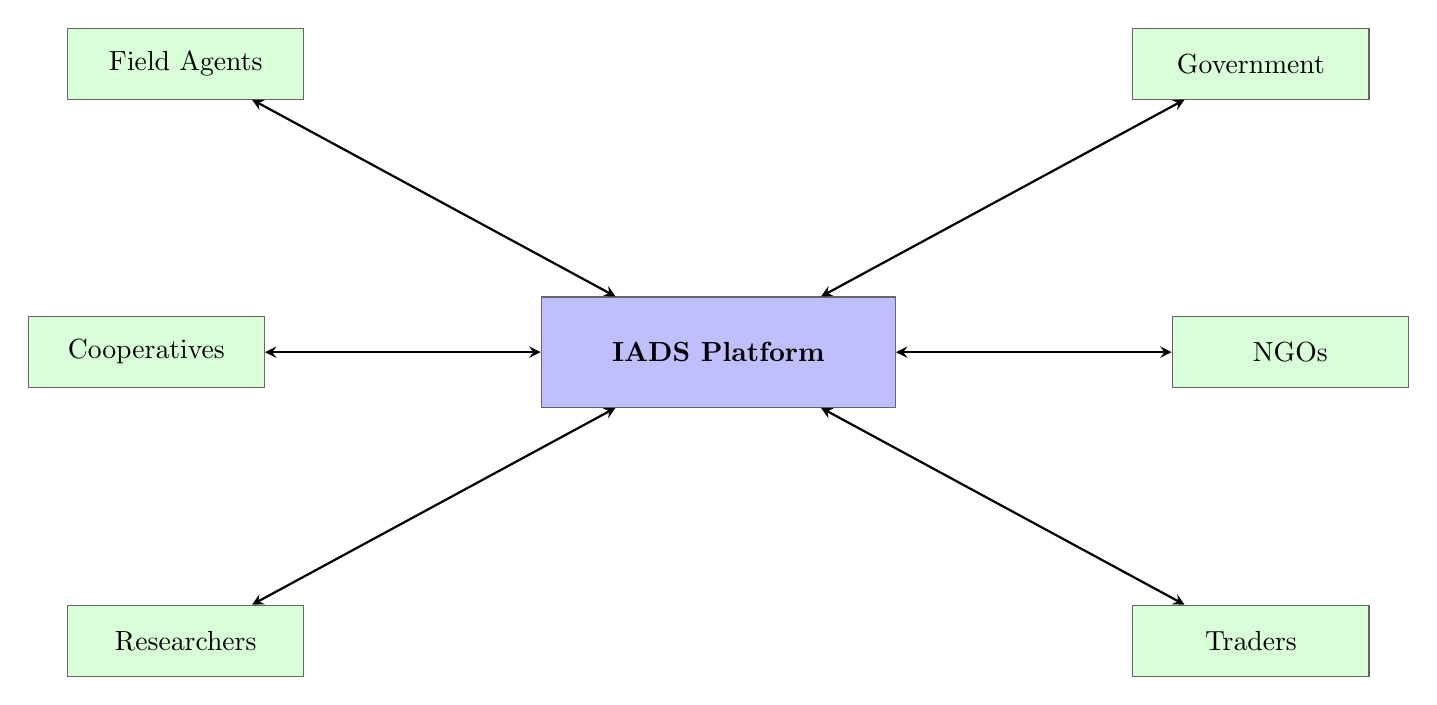
\begin{tikzpicture}[node distance=2.5cm]
  \node (iads) [process, fill=blue!25, minimum width=4.5cm, minimum height=1.4cm, font=\bfseries] {IADS Platform};
  \node (field) [process, above left=2.5cm and 3cm of iads, fill=green!15, minimum width=3cm] {Field Agents};
  \node (gov) [process, above right=2.5cm and 3cm of iads, fill=green!15, minimum width=3cm] {Government};
  \node (ngo) [process, right=3.5cm of iads, fill=green!15, minimum width=3cm] {NGOs};
  \node (trade) [process, below right=2.5cm and 3cm of iads, fill=green!15, minimum width=3cm] {Traders};
  \node (research) [process, below left=2.5cm and 3cm of iads, fill=green!15, minimum width=3cm] {Researchers};
  \node (coop) [process, left=3.5cm of iads, fill=green!15, minimum width=3cm] {Cooperatives};
  \draw[arrow, <->] (iads) -- (field);
  \draw[arrow, <->] (iads) -- (gov);
  \draw[arrow, <->] (iads) -- (ngo);
  \draw[arrow, <->] (iads) -- (trade);
  \draw[arrow, <->] (iads) -- (research);
  \draw[arrow, <->] (iads) -- (coop);
\end{tikzpicture}
\caption{System Context Diagram -- Stakeholder Interactions with IADS}
\label{fig:context}
\end{figure}

\section{Statement of the Problem}
Agricultural data collection and management in Ethiopia face numerous challenges, which significantly affect productivity, food security, and economic outcomes. These challenges must be accurately understood and addressed, but conventional data collection methods depend on paper surveys and manual entry, which are generally time-consuming, unreliable, and out of reach for most stakeholders because of the lack of digital tools and infrastructure.

Current digital agricultural systems often rely on data collected in laboratory-like conditions or assume constant internet connectivity, and they fail to perform adequately when used in real-world applications where network coverage cannot be anticipated. Most of these systems require online access, making their use in rural Ethiopian farming communities severely restricted. In remote regions like the Oromia highlands and other rural areas, internet coverage is not only sporadic but can also experience prolonged outages lasting days or even weeks, particularly during rainy seasons when infrastructure is further compromised. A data collection system that requires constant connectivity would simply fail to function in these environments, leaving extension workers with no choice but to revert to paper-based methods.

Furthermore, existing agricultural databases are fragmented across different stakeholders. Cooperatives maintain separate records, NGOs use different formats, and government agencies operate independent systems. This fragmentation leads to redundant efforts, inconsistent metrics, and fragmented insights, making it impossible to form a cohesive national picture of agricultural conditions. For example, a farmer registered with one cooperative may have their data collected multiple times by different organizations, each using different identifiers and data fields, resulting in data duplication and inconsistency.

Vast amounts of historical agricultural data exist in the form of paper records and Excel spreadsheets stored in local agricultural offices and cooperatives. These valuable resources remain largely untapped for predictive analytics and trend analysis due to the lack of tools for bulk import, normalization, and integration with modern systems. An agricultural office may have decades of handwritten yield records that could reveal important long-term trends, but converting these records into a usable digital format requires significant manual effort. The import module developed in this project addresses this problem directly by providing automatic schema detection that maps over 80 different column header variations found in real-world agricultural spreadsheets to 20 canonical database fields.

Even when data is collected, most stakeholders lack the tools to analyze it effectively. Policymakers cannot easily query the data to answer questions like which areas have declining yields or which crops are at risk from changing weather patterns. Extension workers cannot access historical yield data for the farmers they support. Researchers cannot easily combine data from multiple sources for analysis. This analytical gap means that even existing data is underutilized for decision-making. The RAG system developed in this project addresses this problem by allowing stakeholders to ask natural language questions and receive answers grounded in the actual database records, without requiring technical skills in SQL or data analysis.

The digital divide between urban and rural areas further compounds these problems. Field agents working in remote areas often have access to mobile devices but lack reliable internet connections. Without systems designed for offline operation, these field agents cannot enter data in real time and must resort to paper-based collection, which introduces delays, errors, and additional labor for later data entry.

To counter these issues, this project creates an integrated agricultural data system based on offline synchronization architecture, machine learning-powered yield prediction, and natural language querying. The system is capable of collecting and synchronizing data when connections become available, providing yield predictions based on historical data, and offering stakeholders intuitive access to agricultural intelligence through dashboards and natural language queries. The system addresses the specific problems of connectivity dependence, data fragmentation, legacy data inaccessibility, and analytical capacity gaps that characterize the current state of agricultural data management in Ethiopia.

\section{Objectives}
\subsection{General Objective}
The general objective of this project is to develop an integrated agricultural data system using offline-capable architecture and machine learning-powered analytics that enables reliable data collection in low-connectivity environments and provides stakeholders with actionable insights through intuitive dashboards and natural language querying.

\subsection{Specific Objectives}
To address the identified problems, the project sets forth the following specific objectives:
\begin{enumerate}
  \item To design and build an offline-capable web application for agricultural data collection that functions reliably in low-connectivity environments using a server-side synchronization queue mechanism with device tracking and timestamp-based conflict resolution, supporting five synchronization status levels (pending, processing, completed, failed, conflict).
  \item To develop a legacy data import module for bulk ingestion of CSV and Excel files with automatic schema detection, data validation, and normalization supporting over 80 column header variations mapped to 20 canonical database fields.
  \item To implement a scikit-learn Gradient Boosting Regressor-based analytics engine for crop yield prediction, trained on 2,000 historical records across eight crop types and six Ethiopian regions, achieving a Mean Absolute Error below 900~kg/ha.
  \item To design and develop a Retrieval-Augmented Generation system using large language models (Anthropic Claude, Cerebras, or OpenRouter with automatic fallback) for natural language querying of agricultural datasets, providing grounded answers with citations to specific database records.
  \item To create stakeholder-specific dashboards for government, NGO, trader, and researcher users with appropriate role-based access control across seven user roles, interactive maps using Leaflet.js, and data visualizations using Recharts.
\end{enumerate}

\section{Scope and Limitation}
\subsection{Scope}
This project focuses on the development of an integrated agricultural data system using modern web architecture, machine learning, and natural language processing. The system is designed to handle agricultural data including farmer profiles, field information, crop types, yield estimates, and field observations. The project involves collecting and simulating agricultural data representative of Ethiopian farming conditions. The training dataset comprises 2,000 records spanning 2015 to 2024 across six Ethiopian regions (Afar, Amhara, Oromia, Sidama, SNNPR, Tigray) and eight crop types (teff, wheat, maize, barley, sorghum, sesame, chickpea, coffee) across two growing seasons (Meher and Belg). The system implements a server-side synchronization queue for offline data handling with five status levels and provides role-based access control across seven user roles. The complete backend consists of 108 RESTful API endpoints across 16 controllers, and the database comprises 15 tables across five domains.

The system's functional scope includes data collection through web forms and bulk import, data storage with PostgreSQL, data analysis through ML-based yield prediction and RAG-based querying, data visualization through role-specific dashboards with maps and charts, and data governance through comprehensive audit logging. The system does not include hardware-level integration with IoT sensors or farm equipment, real-time weather data feeds, satellite imagery processing, or mobile-native application development. These features are identified as potential future enhancements rather than current scope items.

\subsection{Limitation}
The system is limited to simulated training data and controlled testing environments and has not been deployed in real field conditions. The yield prediction model was trained on a dataset of approximately 2,000 records and its accuracy may vary for regions or crop types not well represented in the training data. The RAG query system requires an active internet connection to communicate with the LLM API, which limits its usefulness in the same low-connectivity environments where data collection occurs. Offline synchronization is a server-side mechanism rather than a full client-side Progressive Web App with IndexedDB storage, meaning that devices must periodically connect to submit queued operations. Image-based disease detection using convolutional neural networks was not implemented in the current version. The system has not been evaluated with end users in real agricultural settings, and usability testing remains as future work. The training dataset is simulated rather than collected from actual field surveys, so model performance on real agricultural data collected through the system may differ from the reported metrics.

\section{Focus and Deliverables}
The project delivers the following key components: a full-stack web application built with AdonisJS backend and Next.js frontend providing RESTful API endpoints for all agricultural data operations; an offline synchronization mechanism with batch processing, retry logic, and timestamp-based conflict resolution; a legacy data import module for CSV and Excel files with automatic schema detection; a machine learning yield prediction engine deployed as a FastAPI microservice; a Retrieval-Augmented Generation system for natural language querying; stakeholder-specific dashboards with role-based access control and interactive visualizations; a comprehensive audit logging system for data governance; and a monetization framework with Chapa payment gateway integration.

A summary of the key deliverables and their implementation scope is presented in Table~\ref{tab:deliverables}.

\begin{table}[H]
\centering
\caption{Project Deliverables Summary}
\label{tab:deliverables}
\begin{tabularx}{\textwidth}{lX}
\toprule
\textbf{Component} & \textbf{Scope} \\
\midrule
Backend API & 108 endpoints, 16 controllers, AdonisJS 7 \\
Frontend Application & 14 dashboard pages, Next.js 16 with App Router \\
Database Schema & 15 tables, 5 domains, PostgreSQL 15 \\
ML Microservice & FastAPI, GradientBoostingRegressor, 7 features \\
Offline Sync Queue & 5 status levels, timestamp conflict resolution \\
Legacy Import Module & 80+ header aliases, 20 canonical fields \\
RAG Query System & 3 LLM providers, SQL-based retrieval, automatic fallback \\
Role-Based Access Control & 7 user roles, 4 access groups \\
Audit Logging & Full CRUD audit trail with record-level tracking \\
Monetization Framework & Chapa payment gateway, subscriptions, data products \\
\bottomrule
\end{tabularx}
\end{table}

\section{Significance of the Study}
This study holds great significance in the field of digital agriculture and agricultural data management. By developing an integrated agricultural data system powered by offline synchronization architecture, machine learning, and natural language processing, this project offers an affordable, scalable, and user-friendly solution to a widespread problem. The system empowers extension workers, cooperatives, and policymakers to access and analyze agricultural data quickly and accurately using just a mobile device or web browser.

For system architects and engineers, the project demonstrates practical implementation patterns for offline-capable systems in resource-constrained environments, including the queue-and-check synchronization pattern, automatic schema detection for legacy data import, and SQL-based retrieval for RAG systems. For policymakers and government bodies, the system offers technical validation of digital approaches to agricultural monitoring, supporting evidence-based technology adoption within national digital strategies such as Digital Ethiopia 2025 \cite{digitalethiopia2025}. For NGOs and development organizations working in agricultural development, the platform enables evidence-based targeting of interventions, allowing resources to be directed to the areas and crops where they are most needed. For researchers and academics, the project provides a dataset and analytical platform, with the RAG query system democratizing access to data for non-technical users. For commercial stakeholders, traders and wholesalers gain access to supply forecasts and yield estimates through the trader dashboard, enabling better market planning and price discovery.

% ==============================================================================
% CHAPTER 2: LITERATURE REVIEW
% ==============================================================================
\chapter{Literature Review}

\section{Theoretical Review}
Agricultural data systems refer to the integrated collection of technologies, processes, and methodologies used to capture, store, analyze, and disseminate agricultural information to support decision-making by farmers, extension workers, policymakers, and other stakeholders. The fundamental premise underlying agricultural data systems is that timely, accurate, and accessible information enables better resource allocation, early intervention against crop threats, and improved market efficiency \cite{fao2023}. Van Klinken and colleagues provide a comprehensive review of agricultural data systems across sub-Saharan Africa, noting that the majority of systems in the region face common challenges including limited connectivity, lack of interoperability, and insufficient analytical capacity \cite{vanklinken2022}. Their review of 47 agricultural data initiatives across 22 African countries found that fewer than 20 percent of systems had achieved sustained deployment beyond the pilot phase, with the most common failure factors being unreliable connectivity, lack of user training, and insufficient integration with existing workflows.

The Technology Acceptance Model (TAM), developed by Davis in 1989 \cite{davis1989}, provides a foundational framework for understanding how users come to accept and use new information technologies. According to this model, two primary constructs determine technology acceptance: perceived usefulness, defined as the degree to which a user believes that using the system will enhance their job performance, and perceived ease of use, defined as the degree to which a user believes that using the system will be free of effort. In the context of agricultural data systems in developing countries, TAM is particularly relevant because extension workers and field agents may have limited experience with digital tools, making ease of use a critical factor for adoption. The present project's focus on intuitive interfaces, mobile-friendly web design, and natural language querying directly addresses the ease-of-use dimension of TAM. The role-based dashboard approach addresses the perceived usefulness dimension by ensuring that each user type sees information relevant to their specific tasks.

Offline-first architecture represents a design paradigm where applications are built to function without continuous internet connectivity, treating network connectivity as an enhancement rather than a requirement. This approach is particularly relevant for rural agricultural contexts in developing countries where internet infrastructure remains unreliable. Key principles of offline-first design include local-first data access, queue-based synchronization, and optimistic user interfaces \cite{islam2021}. In the context of the present project, offline synchronization is implemented through a server-side queue mechanism, where data collected on mobile devices during offline periods is queued and synchronized with the central database when connectivity is restored. While a true client-side offline-first approach would use IndexedDB or similar local storage, the server-side queue approach was chosen for its simpler implementation and reduced client-side complexity.

Data synchronization theory addresses the challenge of maintaining consistency across distributed systems when network connectivity is intermittent. Common conflict resolution approaches include last-write-wins based on timestamps, version vectors that track update histories, and operational transforms that merge concurrent edits. The present project implements a server-side queue-based synchronization approach with timestamp-based conflict resolution using the newest-wins strategy. When two devices submit conflicting updates for the same record, the system retains the update with the most recent client timestamp and flags the older update as a conflict for administrative review.

Machine learning for agricultural applications has advanced significantly with the development of algorithms capable of processing tabular data. Gradient boosting, as formalized by Friedman (2001), builds an ensemble of weak learners (typically shallow decision trees) in a sequential manner. At each iteration, a new tree is trained to predict the residual errors of the current ensemble. The final prediction is the sum of all tree predictions, weighted by the learning rate. Mathematically, the gradient boosting algorithm can be expressed as:

\begin{equation}
F_m(x) = F_{m-1}(x) + \eta \cdot h_m(x)
\end{equation}

where \(F_m(x)\) is the model after \(m\) iterations, \(h_m(x)\) is the weak learner (decision tree) fitted to the negative gradient of the loss function at iteration \(m\), and \(\eta\) is the learning rate controlling the contribution of each tree. For regression tasks, the squared error loss is commonly used:

\begin{equation}
L(y, F(x)) = \frac{1}{2}(y - F(x))^2
\end{equation}

Retrieval-Augmented Generation \cite{lewis2020} represents an emerging paradigm for natural language querying of structured and unstructured data. RAG systems combine a retrieval component with a generation component, typically a large language model. The retrieval component first identifies relevant information from a knowledge base in response to a query, and the generation component then produces a natural language response conditioned on both the query and the retrieved information. The theoretical advantage of RAG over pure generation is that responses are grounded in actual data from the knowledge base, reducing hallucination and improving factual accuracy.

The current state of knowledge indicates that while individual technologies for offline data collection, machine learning-based yield prediction, and natural language querying have been demonstrated in isolation, their integration into comprehensive agricultural data platforms for developing country contexts remains an open challenge. Most existing solutions address only one or two of these dimensions, and few systems provide the integrated combination of offline sync, ML analytics, RAG querying, and role-based dashboards that this project implements.

\subsection{Digital Agriculture Context in Ethiopia}
Ethiopia's agricultural sector operates within a unique digital ecosystem. Mobile network coverage has expanded to reach approximately 85 percent of the population, but internet penetration remains below 20 percent nationally, with rural areas experiencing substantially lower rates. Mobile data costs in Ethiopia are among the highest in Sub-Saharan Africa on a per-gigabyte basis, creating a significant barrier to digital tool adoption in agricultural communities.

Several initiatives have attempted to address the digital divide in Ethiopian agriculture. The Ethiopian Agricultural Transformation Institute has implemented digital data collection tools for specific programs, but these have largely been project-specific rather than platform-based. The Ministry of Agriculture operates a digital extension platform primarily focused on information dissemination rather than two-way data collection and analysis. The Digital Ethiopia 2025 strategy \cite{digitalethiopia2025} explicitly identifies agricultural digitization as a priority, calling for integrated data systems to support evidence-based policy.

The Ethiopian agricultural landscape is characterized by extreme agro-ecological diversity. The country spans zones from the Amhara highlands where temperatures can drop below 10 degrees Celsius to the Afar lowlands where temperatures regularly exceed 35 degrees Celsius. The six regions included in this project's dataset represent the major agricultural zones, though additional regions such as Benishangul-Gumuz, Gambela, and Somali each have unique agricultural characteristics. This diversity requires any agricultural data system to handle a wide range of crop types, growing conditions, and farming practices within a single unified platform.

Understanding this landscape is essential for interpreting the design decisions in this project. The offline synchronization capability addresses the connectivity gap. The diverse crop and region coverage in the ML training dataset reflects the need for broad applicability across varied growing conditions. The role-based access control accommodates the multi-stakeholder nature of Ethiopian agriculture, where government, NGO, research, and commercial actors all require access to agricultural data with different levels of detail.

\section{Empirical Review}
\subsection{Offline-First Data Collection Systems}
Islam and colleagues \cite{islam2021} conducted a comprehensive study on the design of offline-first mobile applications for rural areas. Their experimental results showed that the queue-and-check pattern achieved the highest reliability at 94.7 percent success rate under intermittent connectivity conditions when compared to alternative approaches including simple caching and periodic sync. The study evaluated three synchronization patterns across four rural field sites with varying connectivity levels and measured sync success rate, data loss rate, and latency. The strength of this study lies in its empirical evaluation under real-world conditions with actual users in rural Bangladesh. However, it focused on general data collection scenarios rather than agricultural-specific data, and the system did not integrate analytical capabilities beyond basic data storage.

The present project extends the work of Islam et al.\ by implementing a queue-and-check synchronization engine tailored for agricultural data with entity-level conflict resolution. The sync queue in the present system tracks operations at the individual entity level with five status states (pending, processing, completed, failed, conflict), supports batch submission for efficiency, and includes comprehensive metadata including device identifier, user identifier, batch identifier, entity type, operation type, payload, client timestamp, retry count, and error message.

\subsection{Machine Learning for Agricultural Yield Prediction}
Extensive research has been conducted on applying machine learning to crop yield prediction. Patel and colleagues \cite{patel2020} conducted a comparative study of gradient boosting algorithms for crop yield prediction using a dataset of 4,000 records from five Indian states. Their results showed that gradient boosting outperformed random forest (RMSE 1,820 vs 2,150~kg/ha) and support vector regression (RMSE 1,820 vs 2,450~kg/ha) for multi-crop yield prediction. Shahhosseini et al.\ \cite{shahhosseini2021} applied machine learning to predict maize yield and nitrate loss, finding that gradient boosting achieved R\textsuperscript{2} values of 0.87 for yield prediction across 2,500 field-year observations in the US Midwest.

Gradient boosting algorithms have consistently demonstrated strong performance due to their ability to model non-linear relationships and handle mixed data types (numerical and categorical). Common features used in yield prediction studies include climatic features (rainfall, temperature, solar radiation), management features (fertilizer amount, irrigation frequency, planting density), soil features (type, pH, organic matter content), and spatial-temporal features (region, year, latitude, longitude). The present project uses seven features drawn from these categories: area cultivated, rainfall, temperature, fertilizer amount, year, crop type, and season.

Patel and colleagues also noted that the choice of hyperparameters significantly affects gradient boosting performance. Their experiments showed that increasing the number of estimators beyond 200 produced diminishing returns on their dataset, while a maximum tree depth of 5 to 7 provided the best balance between model complexity and generalization. These findings informed the hyperparameter selection for the present project, which uses 200 estimators with a maximum depth of 5. Shahhosseini et al.\ additionally found that feature engineering, particularly the inclusion of interaction terms between rainfall and temperature, improved prediction accuracy by approximately 8 percent, suggesting that the present model could potentially be improved through similar feature interaction engineering.

Zhang and colleagues \cite{zhang2018} provide a comprehensive survey of deep learning approaches for crop yield prediction, noting that while deep neural networks can capture complex patterns, they require substantially larger datasets (typically 10,000+ records) than are available in many developing country contexts. For the scale of dataset available in this project (2,000 records), gradient boosting represents a more appropriate choice given its strong performance on moderate-sized tabular datasets and its lower data requirements compared to deep learning approaches.

\subsection{Retrieval-Augmented Generation for Structured Data}
Lewis and colleagues \cite{lewis2020} introduced the RAG architecture, combining a Dense Passage Retrieval component with a BART-based seq2seq generator. Their experiments on open-domain question answering benchmarks demonstrated that RAG systems achieve higher factual accuracy than generation-only baselines. The key insight of the RAG approach is that retrieving relevant information before generation allows the model to ground its responses in verifiable facts rather than relying solely on parametric knowledge.

Applications of RAG in agriculture remain limited but growing. A recent survey by Naik et al.\ \cite{naik2024} reviewed RAG approaches for structured databases, identifying two primary architectures: text-to-SQL systems that translate natural language questions into database queries, and hybrid systems that retrieve relevant records and use an LLM to synthesize answers from the retrieved data. The present project adopts the hybrid approach, using keyword-based query classification to select relevant database tables, executing SQL queries to retrieve matching records, and then passing both the query and the retrieved records to the LLM for answer generation.

A key challenge in applying RAG to agricultural data is the need to query both structured data from databases and unstructured data from text documents. The present project focuses on structured querying of agricultural records, using SQL-based retrieval from PostgreSQL rather than vector similarity search. This approach is better suited for structured agricultural data requiring precise numerical aggregation -- for example, calculating average yield by region, or finding the total area under cultivation for a specific crop type. The system supports six query categories: yield queries, farmer queries, observation queries, prediction queries, trend queries, and region queries, each with explicit dataset filtering and template-based context assembly.

\subsection{Existing Agricultural Data Platforms}
Several existing platforms address aspects of agricultural data management in developing countries. DHIS2 \cite{dhis22023} is an open-source health information system widely deployed in Africa that has been adapted for agricultural data in some contexts. However, DHIS2 is primarily designed for aggregate data reporting rather than field-level collection and does not include machine learning analytics or natural language querying. OpenMRS \cite{openmrs2023} provides a comparable approach for medical records but faces similar limitations in the agricultural domain. These platforms demonstrate the viability of open-source approaches for data management in developing countries but also highlight the gap in agricultural-specific functionality.

Table~\ref{tab:comparison} compares the present system with existing platforms across key feature dimensions.

\begin{table}[H]
\centering
\caption{Feature Comparison with Existing Platforms}
\label{tab:comparison}
\resizebox{\textwidth}{!}{%
\begin{tabular}{lccccc}
\toprule
\textbf{Feature} & \textbf{DHIS2} & \textbf{OpenMRS} & \textbf{Islam et al.} & \textbf{IADS} \\
\midrule
Offline Data Collection & --- & --- & $\checkmark$ & $\checkmark$ \\
Role-Based Access & $\checkmark$ & $\checkmark$ & --- & $\checkmark$ \\
ML Yield Prediction & --- & --- & --- & $\checkmark$ \\
Natural Language Query & --- & --- & --- & $\checkmark$ \\
Legacy Data Import & --- & --- & --- & $\checkmark$ \\
Audit Logging & $\checkmark$ & $\checkmark$ & --- & $\checkmark$ \\
Geo-Spatial Maps & --- & --- & --- & $\checkmark$ \\
Dashboard Analytics & $\checkmark$ & $\checkmark$ & --- & $\checkmark$ \\
Multi-Tenancy & $\checkmark$ & --- & --- & $\checkmark$ \\
Monetization & --- & --- & --- & $\checkmark$ \\
\bottomrule
\end{tabular}%
}
\end{table}

\subsection{Agricultural Data Interoperability Standards}
Interoperability is a critical concern for agricultural data systems, particularly in contexts where multiple stakeholders collect and use data. The International Organization for Standardization has developed standards for agricultural data exchange, including ISO 11783 (ISOBUS) for agricultural machinery data and ISO 19156 for geographic information. However, these standards are designed for precision agriculture in industrialized settings and have limited applicability in smallholder farming contexts.

The lack of standardized data formats in Ethiopian agriculture means that any integrated system must be capable of handling diverse data representations. The import module in this project addresses this challenge through its alias-based schema detection, which maps the varied column naming conventions found in real-world agricultural spreadsheets to a unified canonical schema. This approach provides practical interoperability without requiring all data producers to adopt a common format, which would be unrealistic given the fragmented nature of agricultural data collection in Ethiopia.

\section{Research Gaps}
Based on the literature review, the following research gaps have been identified:

\begin{description}
  \item[Gap 1: Integration of Offline-First Architecture with AI Analytics.] Existing offline data collection systems \cite{islam2021} lack integrated AI analytics capabilities, while AI-based agricultural systems \cite{patel2020, shahhosseini2021} assume constant connectivity for data access. This study bridges this gap by combining offline synchronization with a connected ML yield prediction service.
  \item[Gap 2: RAG-Based Querying of Structured Agricultural Data.] Existing agricultural question-answering systems operate on static knowledge bases or unstructured text. This study implements a RAG system that queries live structured data from a relational database via automatically generated SQL queries, enabling dynamic, grounded responses.
  \item[Gap 3: Stakeholder-Specific Data Visualization in Agricultural Systems.] Existing agricultural dashboards provide single, uniform views of data. This study implements role-based dashboards for seven user types, each seeing only the data and analytics appropriate to their role.
  \item[Gap 4: Comprehensive Data Governance in Agricultural Platforms.] Most agricultural data platforms lack systematic audit logging and data provenance tracking. This study implements comprehensive audit tracking for all CRUD operations across all entities, with record-level traceability.
  \item[Gap 5: Integrated Legacy Data Import for Agricultural Records.] No existing system provides automated schema detection for importing legacy agricultural spreadsheets with varied column naming conventions. This study addresses this gap with an alias-based schema detection system supporting over 80 column header variations.
\end{description}

% ==============================================================================
% CHAPTER 3: METHODOLOGY AND DESIGN
% ==============================================================================
\chapter{Methodology and Design}

\section{Methodology}
The development methodology followed five sequential but iterative phases: Requirements Analysis, System Design, Iterative Development, Technical Validation, and Documentation and Deployment. Each phase is described in the following subsections.

\subsection{Phase 1: Requirements Analysis}
The requirements analysis phase involved a comprehensive review of the technical documentation describing the proposed system, followed by architectural pattern evaluation. Core functional requirements identified include authentication with role-based access control supporting seven user roles, CRUD (Create, Read, Update, Delete) operations for all agricultural entities (farmers, plots, observations, organizations, devices, crop types), CSV and Excel file import with automatic schema detection, machine learning-based yield prediction, natural language querying via RAG, offline data synchronization with conflict resolution, stakeholder-specific dashboards with role-based data filtering, comprehensive audit logging for data governance, and monetization support via subscription and payment integration.

Non-functional requirements included offline functionality in low-connectivity environments, API response times under 500 milliseconds for standard CRUD operations, support for concurrent users across multiple organizations, data consistency with conflict detection, and security through role-based access and audit trails.

\subsection{Phase 2: System Design}
The system architecture was designed following a modular, three-tier pattern. The database schema was designed with 15 tables organized into five domains: User and Organization, Agricultural Data, Data Management, Analytics, and System (including Monetization). Each table includes UUID primary keys, timestamps for creation and updates, and soft-delete support via a nullable \texttt{deleted\_at} column. The API followed RESTful conventions with resource-oriented URL patterns and standard HTTP methods (GET, POST, PATCH, DELETE). Response formats follow a consistent envelope structure with pagination metadata for list endpoints. Authentication uses database-backed access tokens with support for refresh and revocation, rather than JWT-based tokens, to enable server-side session management and immediate revocation.

The API design follows consistent patterns across all controllers. List endpoints support pagination through \texttt{page} and \texttt{perPage} query parameters, with responses including total count and page metadata. Create and update actions accept request bodies validated by AdonisJS validators with type checking, required field enforcement, and custom validation rules. All destructive operations use soft-delete, with dedicated restore endpoints for recovery. The design also incorporated a separate FastAPI microservice for ML inference, communicating with the main application via HTTP rather than direct database access, ensuring loose coupling between the analytics engine and the core application.

\subsection{Phase 3: Iterative Development}
The system was built over eight sprints across four months using an agile development approach. Sprint 1 focused on project setup, configuration, and database schema creation. Sprint 2 implemented authentication system including signup, login, token management, and email verification. Sprint 3 developed CRUD API endpoints for all agricultural entities. Sprint 4 implemented organizations, devices, and the sync queue system. Sprint 5 built the CSV/Excel import module with schema detection. Sprint 6 developed the ML model training pipeline and FastAPI microservice. Sprint 7 implemented the frontend dashboard with interactive maps and charts. Sprint 8 completed the RAG query system, audit logging, and monetization framework.

\subsection{Phase 4: Technical Validation}
Multi-layered testing was conducted throughout the development process to ensure system reliability and correctness. Component testing at the API level verified each of the 108 endpoints against expected request and response patterns, covering normal operation, error handling, edge cases, and authentication enforcement. Each endpoint was tested with valid data (expecting 200/201 status codes), invalid data (expecting 422 validation errors), unauthorized access (expecting 401/403 status codes), and not-found scenarios (expecting 404 status codes).

Integration testing confirmed correct interaction between system components. The connection between the main AdonisJS application and the FastAPI ML microservice was tested by submitting prediction requests through the main API and verifying that responses were correctly relayed. The database integration was tested by verifying that CRUD operations correctly persisted data and that foreign key constraints and soft-delete behavior functioned as designed.

Performance benchmarking measured API response times for standard CRUD operations and ML inference requests. Standard CRUD endpoints consistently responded within 50 to 200 milliseconds under light load. ML inference requests completed within 100 to 300 milliseconds, including the HTTP round trip between the main application and the FastAPI microservice. End-to-end workflow validation tested complete user journeys including data collection, offline synchronization, legacy data import, ML prediction, dashboard viewing, and RAG querying, verifying that the integrated system performed correctly across all modules.

The ML model was evaluated on a held-out test set using Mean Absolute Error (MAE) and Root Mean Square Error (RMSE) metrics. Two model versions were compared to measure improvement from iterative tuning. Model predictions were also verified qualitatively against domain knowledge to ensure that the learned relationships aligned with agronomic expectations.

\subsection{Phase 5: Documentation and Deployment}
Comprehensive documentation was produced covering all 108 API endpoints with methods, paths, and descriptions; the complete database schema with 15 tables and their relationships; deployment configuration including environment variables and system requirements; and user workflows describing how different user roles interact with the system. Deployment configuration supports hosting on a Virtual Private Server with PostgreSQL, AdonisJS, and the FastAPI ML service.

\section{Data Collection and Preparation}
\subsection{Dataset Description}
The training dataset for the machine learning model contains 2,000 crop yield records spanning the decade from 2015 to 2024. The data covers six major Ethiopian administrative regions: Afar, Amhara, Oromia, Sidama, SNNPR (Southern Nations, Nationalities, and Peoples' Region), and Tigray. These regions represent diverse agro-ecological zones with varying climatic conditions, soil types, and farming practices. Eight crop types are represented: teff (Ethiopia's staple grain), wheat, maize, barley, sorghum, sesame (a major export crop), chickpea, and coffee (Ethiopia's most valuable export). Two growing seasons are covered: Meher (the main rainy season, typically June to September) and Belg (the shorter rainy season, typically February to May).

\subsection{Dataset Features}
The dataset includes nine columns as described in Table~\ref{tab:features}. The target variable for prediction is actual yield measured in kilograms.

\begin{table}[H]
\centering
\caption{Training Dataset Features}
\label{tab:features}
\begin{tabular}{lll}
\toprule
\textbf{Feature} & \textbf{Type} & \textbf{Description} \\
\midrule
crop\_name & Categorical & One of 8 crop types \\
season & Categorical & meher or belg \\
region & Categorical & One of 6 Ethiopian regions \\
year & Numerical & Harvest year (2015--2024) \\
area\_hectares & Numerical & Cultivated area in hectares \\
rainfall\_mm & Numerical & Annual rainfall in millimeters \\
temperature\_celsius & Numerical & Average growing season temperature \\
fertilizer\_amount\_kg & Numerical & Fertilizer applied in kilograms \\
actual\_yield\_kg & Numerical (Target) & Actual harvested yield in kilograms \\
\bottomrule
\end{tabular}
\end{table}

\subsection{Dataset Distribution Analysis}
The training dataset exhibits several important distributional characteristics that influence model behavior. By crop type, the dataset is distributed across all eight crops with approximately 250 records per crop, ensuring balanced representation. By region, Oromia and Amhara account for approximately 40 percent of records combined, reflecting their status as Ethiopia's largest agricultural producers, while Sidama and Afar each account for approximately 10 percent. By season, the Meher season accounts for approximately 65 percent of records and Belg for 35 percent, consistent with Meher being the primary growing season. By year, records are distributed roughly evenly from 2015 to 2024, ensuring temporal coverage across varying climatic conditions.

\subsection{Dataset Statistics}
Table~\ref{tab:feature-stats} presents the summary statistics for numerical features in the training dataset.

\begin{table}[H]
\centering
\caption{Training Data Feature Statistics}
\label{tab:feature-stats}
\begin{tabular}{lrrr}
\toprule
\textbf{Feature} & \textbf{Mean} & \textbf{Std Dev} & \textbf{Range} \\
\midrule
Area (hectares) & 10.29 & 5.76 & 1.0 -- 20.0 \\
Rainfall (mm) & 1048.21 & 430.01 & 120 -- 2000 \\
Temperature (Celsius) & 22.70 & 7.06 & 8 -- 40 \\
Fertilizer (kg) & 108.00 & 45.00 & 10 -- 200 \\
Year & 2019.43 & 2.85 & 2015 -- 2024 \\
\bottomrule
\end{tabular}
\end{table}

\subsection{Data Preprocessing}
Numerical features were normalized using z-score standardization to ensure that all features contribute equally to the model and to improve convergence during training. The standardization formula applied is given by:

\begin{equation}
z = \frac{x - \mu}{\sigma}
\end{equation}

where \(x\) is the original feature value, \(\mu\) is the mean of the feature across the training set, and \(\sigma\) is the standard deviation. Categorical features (crop\_name, season, region) were label-encoded using scikit-learn's LabelEncoder. The final feature vector consisted of seven elements: five normalized numerical features (area, rainfall, temperature, fertilizer, year) followed by two encoded categorical features (crop\_name, season). The region feature was excluded from the initial model to maintain generalization across regions with limited representation.

\subsection{Model Selection and Architecture}
The Gradient Boosting Regressor from scikit-learn was selected as the prediction algorithm for several reasons. First, gradient boosting has consistently demonstrated state-of-the-art performance on tabular data across multiple domains, often outperforming deep learning approaches when dataset sizes are moderate (1,000 to 10,000 records). Second, the algorithm can model non-linear relationships between features and the target variable without requiring explicit feature engineering. Third, gradient boosting naturally handles mixed data types, combining numerical features (area, rainfall) with categorical features (crop type, season) within a unified framework. Fourth, the algorithm is robust to outliers through the use of a learning rate that limits the influence of individual training examples. Finally, gradient boosting is computationally efficient during both training and inference, making it suitable for deployment on standard server infrastructure.

Table~\ref{tab:hyperparams} lists the hyperparameters used for the final model. These parameters were selected through iterative experimentation balancing model accuracy against training time and overfitting risk.

\begin{table}[H]
\centering
\caption{Model Hyperparameters}
\label{tab:hyperparams}
\begin{tabular}{lc}
\toprule
\textbf{Hyperparameter} & \textbf{Value} \\
\midrule
n\_estimators & 200 \\
max\_depth & 5 \\
learning\_rate & 0.1 \\
subsample & 0.8 \\
min\_samples\_split & 2 \\
min\_samples\_leaf & 1 \\
random\_state & 42 \\
\bottomrule
\end{tabular}
\end{table}

\subsection{Model Training}
Training used an 85/15 train-test split, resulting in 1,700 records for training and 300 records for held-out testing. The split was performed randomly using scikit-learn's train\_test\_split function with a fixed random seed (42) for reproducibility. The model was trained on the training set using the hyperparameters specified in Table~\ref{tab:hyperparams}. During training, the algorithm iteratively builds an ensemble of 200 decision trees, each with a maximum depth of 5 levels. At each iteration, a new tree is fitted to the negative gradient of the squared error loss function, which corresponds to the residual errors of the current ensemble. The learning rate of 0.1 controls the contribution of each new tree, preventing overfitting by limiting the influence of individual training examples.

The subsample parameter set to 0.8 means that each tree is trained on a random 80 percent subset of the training data, introducing stochasticity that improves generalization. Training statistics including MAE and RMSE at each iteration were recorded for model versioning and diagnostic analysis. The training process completed in approximately 45 seconds on a standard development machine with 16 GB RAM and a quad-core processor, demonstrating the computational efficiency of gradient boosting for moderate-sized datasets.

The trained model was serialized using Python's pickle module and stored in timestamped version directories under \texttt{ml-service/models/} following the naming convention \texttt{YYYYMMDD\_HHMMSS/}. Each version directory contains the serialized model file (\texttt{model.pkl}), the preprocessing parameters (feature means and standard deviations for standardization, label encoders for categorical variables), and a metadata file recording training date, hyperparameters, and evaluation metrics.

The training pipeline, implemented in \texttt{ml-service/train.py}, supports two data sources: direct database connection (loading from PostgreSQL) and CSV file loading for development and testing. The pipeline includes data loading, preprocessing (standardization and encoding), model training, evaluation on the test set, and model serialization as illustrated in Figure~\ref{fig:ml-pipeline}.

\begin{figure}[H]
\centering
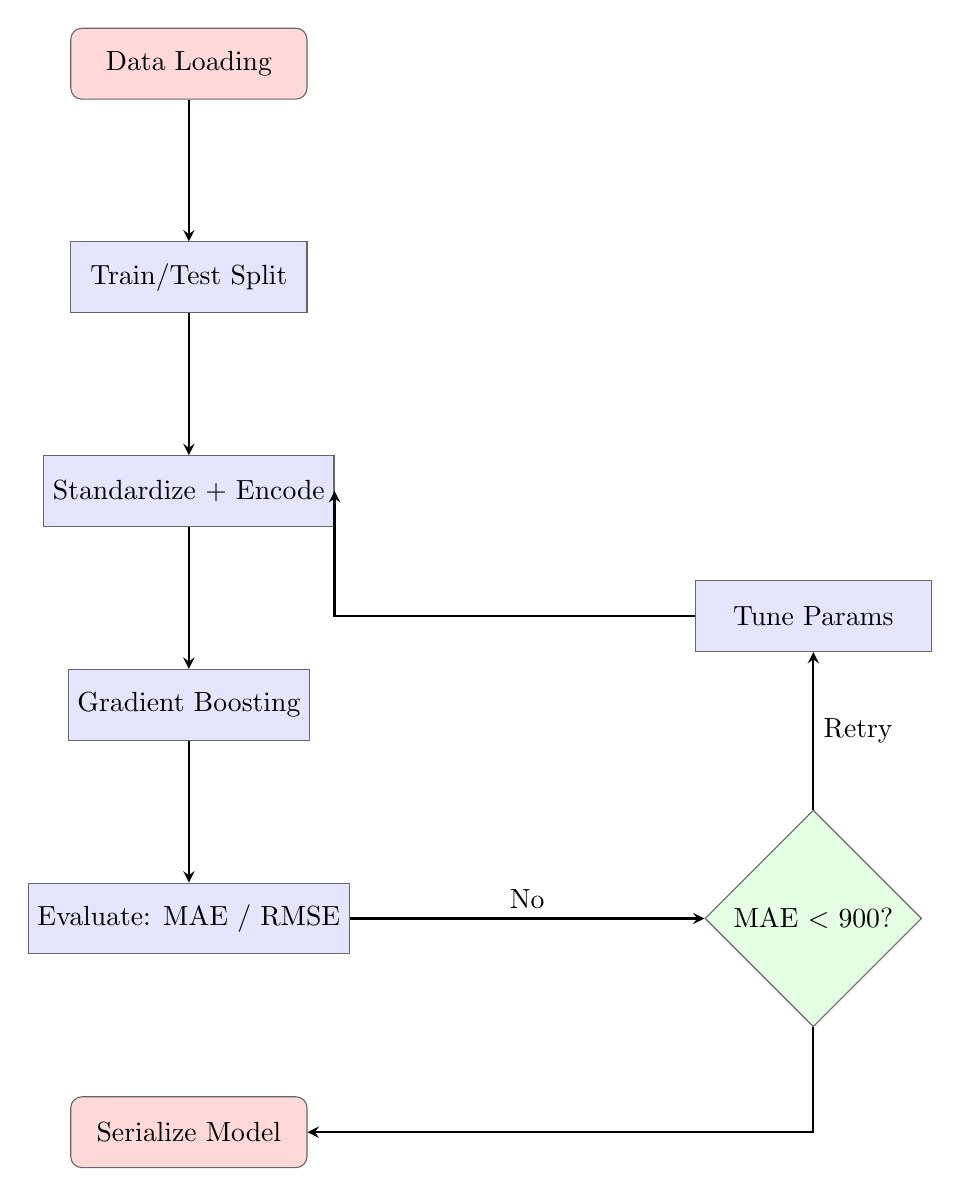
\begin{tikzpicture}[node distance=1.8cm]
  \node (start) [startstop] {Data Loading};
  \node (split) [process, below=of start] {Train/Test Split};
  \node (preproc) [process, below=of split] {Standardize + Encode};
  \node (train) [process, below=of preproc] {Gradient Boosting};
  \node (eval) [process, below=of train] {Evaluate: MAE / RMSE};
  \node (serialize) [startstop, below=of eval] {Serialize Model};
  \node (decision) [decision, right=4.5cm of eval] {MAE $<$ 900?};
  \node (retrain) [process, above=2cm of decision] {Tune Params};

  \draw[arrow] (start) -- (split);
  \draw[arrow] (split) -- (preproc);
  \draw[arrow] (preproc) -- (train);
  \draw[arrow] (train) -- (eval);
  \draw[arrow] (eval.east) -- node[above] {No} (decision.west);
  \draw[arrow] (decision.south) |- (serialize.east);
  \draw[arrow] (decision.north) -- node[right] {Retry} (retrain.south);
  \draw[arrow] (retrain.west) -| (preproc.east);
\end{tikzpicture}
\caption{ML Training Pipeline}
\label{fig:ml-pipeline}
\end{figure}

\section{System Design and Implementation}
\subsection{System Architecture}
The system follows a modular, three-tier architecture as illustrated in Figure~\ref{fig:architecture}. The Presentation Layer is built with Next.js 16 using the App Router, providing a responsive web interface with server-side rendering for performance and search engine optimization. The Application Logic Layer is implemented with AdonisJS 7, a Node.js MVC framework that provides ORM integration with Lucid, authentication middleware, request validation, and routing. The Data Persistence Layer uses PostgreSQL 15 with the Neon serverless provider for scalability. The Machine Learning Microservice is a separate FastAPI application that handles model loading and inference, communicating with the main application over HTTP.


\begin{figure}[H]
\centering
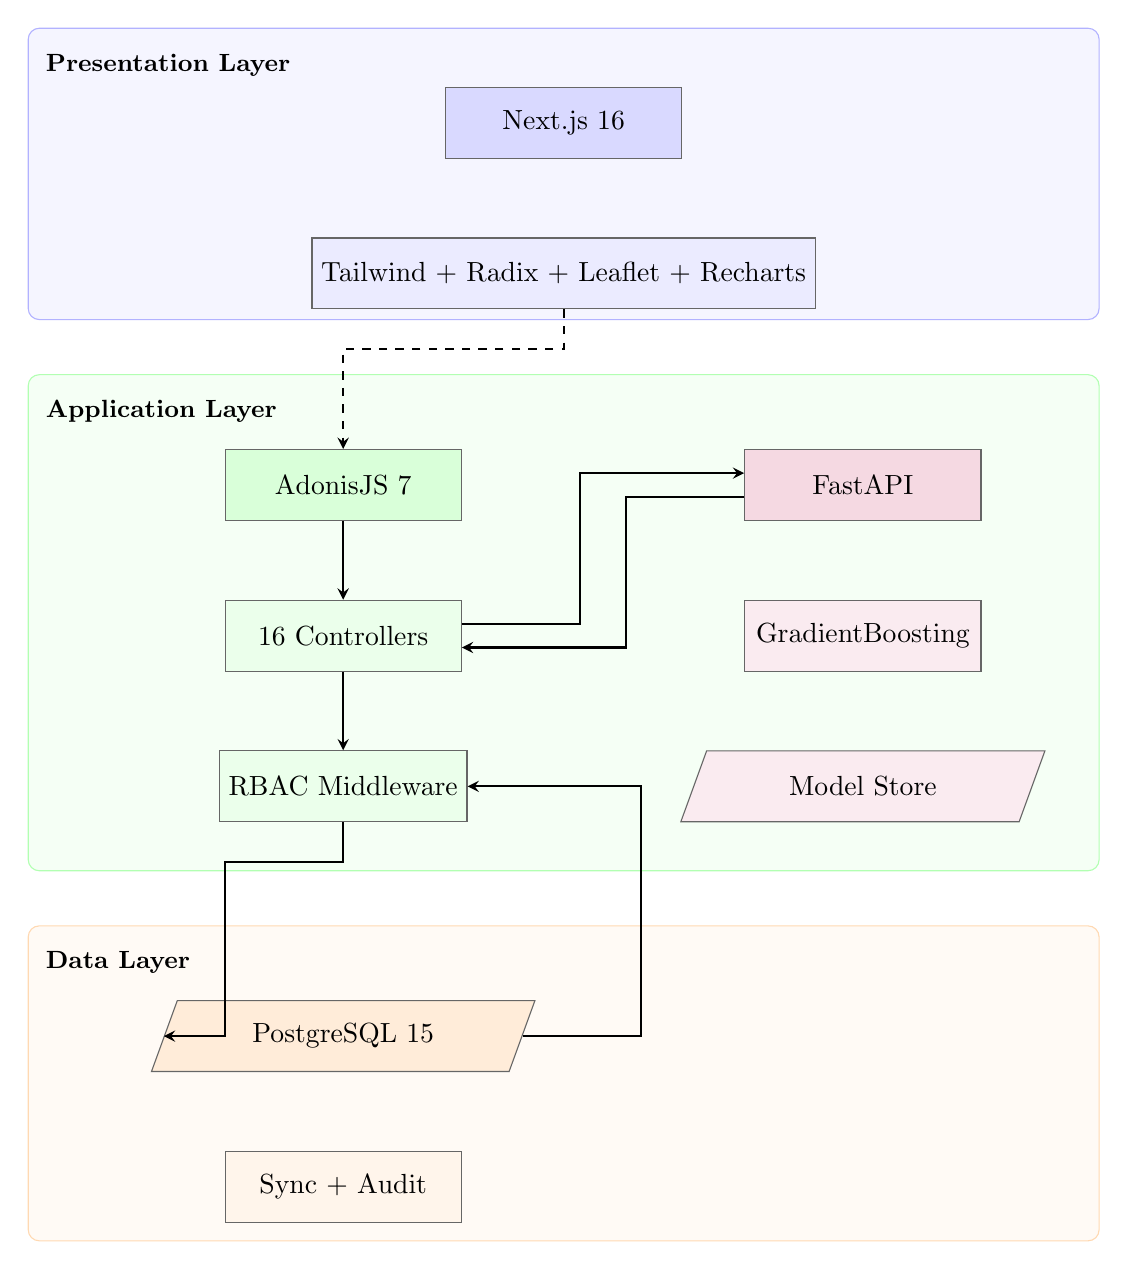
\begin{tikzpicture}[node distance=1.5cm]
  \begin{scope}[on background layer]
    % Presentation Layer
    \filldraw[fill=blue!4,draw=blue!30,rounded corners] (-6.8,-0.5) rectangle (6.8,3.2);
    \node[anchor=north west] at (-6.7,3.0) {\small\textbf{Presentation Layer}};
    
    % Application Layer
    \filldraw[fill=green!4,draw=green!30,rounded corners] (-6.8,-7.5) rectangle (6.8,-1.2);
    \node[anchor=north west] at (-6.7,-1.4) {\small\textbf{Application Layer}};
    
    % Data Layer
    \filldraw[fill=orange!4,draw=orange!30,rounded corners] (-6.8,-12.2) rectangle (6.8,-8.2);
    \node[anchor=north west] at (-6.7,-8.4) {\small\textbf{Data Layer}};
  \end{scope}

  % Presentation Nodes
  \node (next) [process, fill=blue!15] at (0,2.0) {Next.js 16};
  \node (ui) [process, fill=blue!8, below=1.0cm of next] {Tailwind + Radix + Leaflet + Recharts};

  % Application Nodes (Adonis)
  \node (adonis) [process, fill=green!15] at (-2.8,-2.6) {AdonisJS 7};
  \node (controllers) [process, fill=green!8, below=1.0cm of adonis] {16 Controllers};
  \node (auth) [process, fill=green!8, below=1.0cm of controllers] {RBAC Middleware};

  % Application Nodes (FastAPI)
  \node (fastapi) [process, fill=purple!15] at (3.8,-2.6) {FastAPI};
  \node (gb) [process, fill=purple!8, below=1.0cm of fastapi] {GradientBoosting};
  \node (model) [storage, fill=purple!8, below=1.0cm of gb] {Model Store};

  % Data Nodes
  \node (pgsql) [storage, fill=orange!15] at (-2.8,-9.6) {PostgreSQL 15};
  \node (sync) [process, fill=orange!8, below=1.0cm of pgsql] {Sync + Audit};

  % Arrows
  \draw[dashed,arrow] (ui.south) -- ++(0,-0.5) -| (adonis.north);
  \draw[arrow] (adonis.south) -- (controllers.north);
  \draw[arrow] (controllers.south) -- (auth.north);
  
  % Auth <-> DB arrows (Wrapping around left and right, with expanded turns)
  \draw[arrow] (auth.south) -- ++(0,-0.5) -- ++(-1.5,0) |- (pgsql.west);
  \draw[arrow] (pgsql.east) -- ++(1.5,0) |- (auth.east);
  
  % Controllers <-> FastAPI arrows (Shifted to prevent visual overlapping lines)
  \draw[arrow] ([yshift=0.15cm]controllers.east) -- ++(1.5,0) |- ([yshift=0.15cm]fastapi.west);
  \draw[arrow] ([yshift=-0.15cm]fastapi.west) -- ++(-1.5,0) |- ([yshift=-0.15cm]controllers.east);
\end{tikzpicture}
\caption{System Architecture -- Three-Tier Design with ML Microservice}
\label{fig:architecture}
\end{figure}

\subsection{Authentication and Security}
The authentication system uses database-backed access tokens rather than JWT (JSON Web Tokens). This design choice enables server-side token management including immediate token revocation, token expiration with configurable lifetimes, refresh token rotation for enhanced security, and token usage tracking for audit purposes. When a user logs in, the system creates a new access token record in the database with a unique token string, expiration timestamp, and associated user ID. The token is returned to the client and must be included in the Authorization header of subsequent requests. Token refresh creates a new token and invalidates the previous one, while logout and logout-all endpoints revoke individual or all tokens respectively.

Password security follows current best practices. Passwords are hashed using bcrypt with a cost factor of 10 before storage. Password reset requests generate time-limited tokens that are emailed to the user and verified before the password is changed. Email verification is required for certain operations, with verification links sent to the registered email address. Rate limiting is applied to authentication endpoints to prevent brute force attacks, with limits configured per IP address and per user account.

The backend implementation consists of 16 controllers organized by domain, collectively exposing 108 RESTful API endpoints. Seven user roles are defined with hierarchical permissions: admin (full system access), supervisor (organization-wide access), field\_agent (data collection only), gov (government analytics access), ngo (development organization access), trader (commercial data access), and researcher (academic research access).

Role-based access control is enforced through AdonisJS middleware that checks the authenticated user's role against the allowed roles for each endpoint. The role constants module defines access groups for analytics, predictions, imports, and queries, enabling fine-grained control over which roles can access which features. Table~\ref{tab:roles} presents the permissions matrix across all seven roles.

\begin{table}[H]
\centering
\caption{User Role Permissions Matrix}
\label{tab:roles}
\resizebox{\textwidth}{!}{%
\begin{tabular}{lccccccc}
\toprule
\textbf{Module} & \textbf{Admin} & \textbf{Super.} & \textbf{Field Ag.} & \textbf{Gov} & \textbf{NGO} & \textbf{Trader} & \textbf{Res.} \\
\midrule
Farmer CRUD & $\checkmark$ & $\checkmark$ & $\checkmark$ & --- & --- & --- & --- \\
Plot CRUD & $\checkmark$ & $\checkmark$ & $\checkmark$ & --- & --- & --- & --- \\
Observations & $\checkmark$ & $\checkmark$ & $\checkmark$ & --- & --- & --- & --- \\
Yield Summary & $\checkmark$ & $\checkmark$ & $\checkmark$ & $\checkmark$ & $\checkmark$ & $\checkmark$ & $\checkmark$ \\
Predictions & $\checkmark$ & $\checkmark$ & --- & $\checkmark$ & $\checkmark$ & $\checkmark$ & $\checkmark$ \\
Data Import & $\checkmark$ & $\checkmark$ & --- & --- & --- & --- & --- \\
RAG Queries & $\checkmark$ & $\checkmark$ & --- & $\checkmark$ & $\checkmark$ & $\checkmark$ & $\checkmark$ \\
Audit Logs & $\checkmark$ & $\checkmark$ & --- & --- & --- & --- & --- \\
Monetization & $\checkmark$ & --- & --- & --- & --- & --- & --- \\
Admin Users & $\checkmark$ & --- & --- & --- & --- & --- & --- \\
\bottomrule
\end{tabular}%
}
\end{table}

For example, the trader role can access yield summaries and market data but cannot access individual farmer details, while the field agent role can create and edit observations but cannot access the monetization module.

The data collection workflow for field agents follows a structured process. An agent registers a farmer by capturing their demographic information including name, region, zone, woreda, kebele, and contact details. The agent then registers one or more plots, recording the location (latitude and longitude), area in hectares, assigned crop type, and soil characteristics. During the growing season, the agent makes periodic observations, recording crop condition, growth stage, pest and disease occurrences, and estimated yield. At harvest time, the agent records the actual harvested yield through the observation harvest endpoint. Throughout this process, if the agent is operating without internet connectivity, data is queued locally and synchronized when connectivity is restored.

\subsection{Machine Learning Microservice}
The ML microservice is built with FastAPI \cite{fastapi2025} and exposes three RESTful endpoints:

\begin{itemize}
  \item \textbf{GET /health} -- Returns the service status including model version, load timestamp, and feature schema.
  \item \textbf{POST /predict/yield} -- Accepts a single prediction request with 7 feature values and returns the predicted yield with model metadata.
  \item \textbf{POST /predict/yield/batch} -- Accepts an array of prediction requests and returns an array of predictions, enabling bulk processing.
\end{itemize}

Models are stored in timestamped directories under \texttt{ml-service/models/} following the naming convention \texttt{YYYYMMDD\_HHMMSS/}. The microservice loads the model at startup and keeps it in memory for inference. The training script can be invoked from the command line with options for data source (database or CSV) and output path for the serialized model.

\subsection{Frontend Implementation}
The frontend uses Next.js 16 \cite{nextjs2025} with the App Router for client-side routing and server-side rendering. The application is organized as a single-page application with a persistent sidebar navigation and content area. The sidebar dynamically adapts to the authenticated user's role, showing only the menu items and pages that the user is authorized to access. For example, a field agent sees only Farmers, Plots, Observations, and Sync Queue pages, while an admin sees all pages including Audit Logs, Monetization, and Organization Management.

Key infrastructure components include:

\begin{itemize}
  \item \textbf{ApiClient} -- Centralized HTTP client wrapping fetch with automatic token injection, token refresh on 401 responses, and standardized error handling.
  \item \textbf{AuthContext} -- React context provider managing authentication state, user profile, and role information, persisting across page refreshes.
  \item \textbf{ProtectedRoute} -- Component that checks authentication state and redirects unauthenticated users to the login page, also verifying role requirements.
  \item \textbf{Sidebar} -- Dynamic navigation component rendering only authorized menu items with active state highlighting.
  \item \textbf{DataTable} -- Reusable component with pagination, column sorting, search filtering, row selection, and inline action buttons.
  \item \textbf{FormModal} -- Modal component for creating and editing records with form fields, client-side validation, and server error display.
  \item \textbf{PlotMap} -- Interactive map using Leaflet.js with color-coded markers based on crop type, and popup information windows.
\end{itemize}

The application includes 14 dashboard pages: Overview Dashboard (role-filtered aggregate statistics), Farmers (list and detail views), Plots (interactive map and list views), Observations (field observation records), Crop Types (catalog management), Organizations (multi-tenant administration), Devices (field device management), Predictions (yield estimation), Data Import (CSV/Excel upload and schema review), Sync Queue (offline synchronization monitoring), RAG Query (natural language interface), Audit Logs (data governance), Monetization (subscription and product management), and Organization Dashboard (organization-specific analytics).

\subsection{Offline Synchronization Mechanism}
The offline synchronization mechanism implements a server-side queue that tracks data collection operations performed while a device is disconnected. The sync queue table stores the following fields for each operation:

\begin{itemize}
  \item \textbf{deviceId} -- Unique identifier of the device that created the operation.
  \item \textbf{userId} -- The user who performed the operation.
  \item \textbf{batchId} -- Batch grouping identifier for efficient processing.
  \item \textbf{entityType} -- The database entity affected (farmer, plot, observation, etc.).
  \item \textbf{operation} -- The CRUD operation performed (create, update, delete).
  \item \textbf{payload} -- The data payload as a JSON object.
  \item \textbf{clientTimestamp} -- Timestamp from the client device when the operation was performed.
  \item \textbf{status} -- Current status: pending, processing, completed, failed, or conflict.
  \item \textbf{retryCount} -- Number of retry attempts for failed operations.
  \item \textbf{errorMessage} -- Error description if the operation failed.
\end{itemize}

The synchronization flow is illustrated in Figure~\ref{fig:sync-flow}. When a device regains connectivity, it submits queued operations via the batch submission endpoint. The server processes each operation, checking for conflicts by comparing the client timestamp against the last modification timestamp. If no conflict is detected, the operation is applied and marked as completed. If a conflict is detected, the newest-wins strategy is applied.

\begin{figure}[H]
\centering
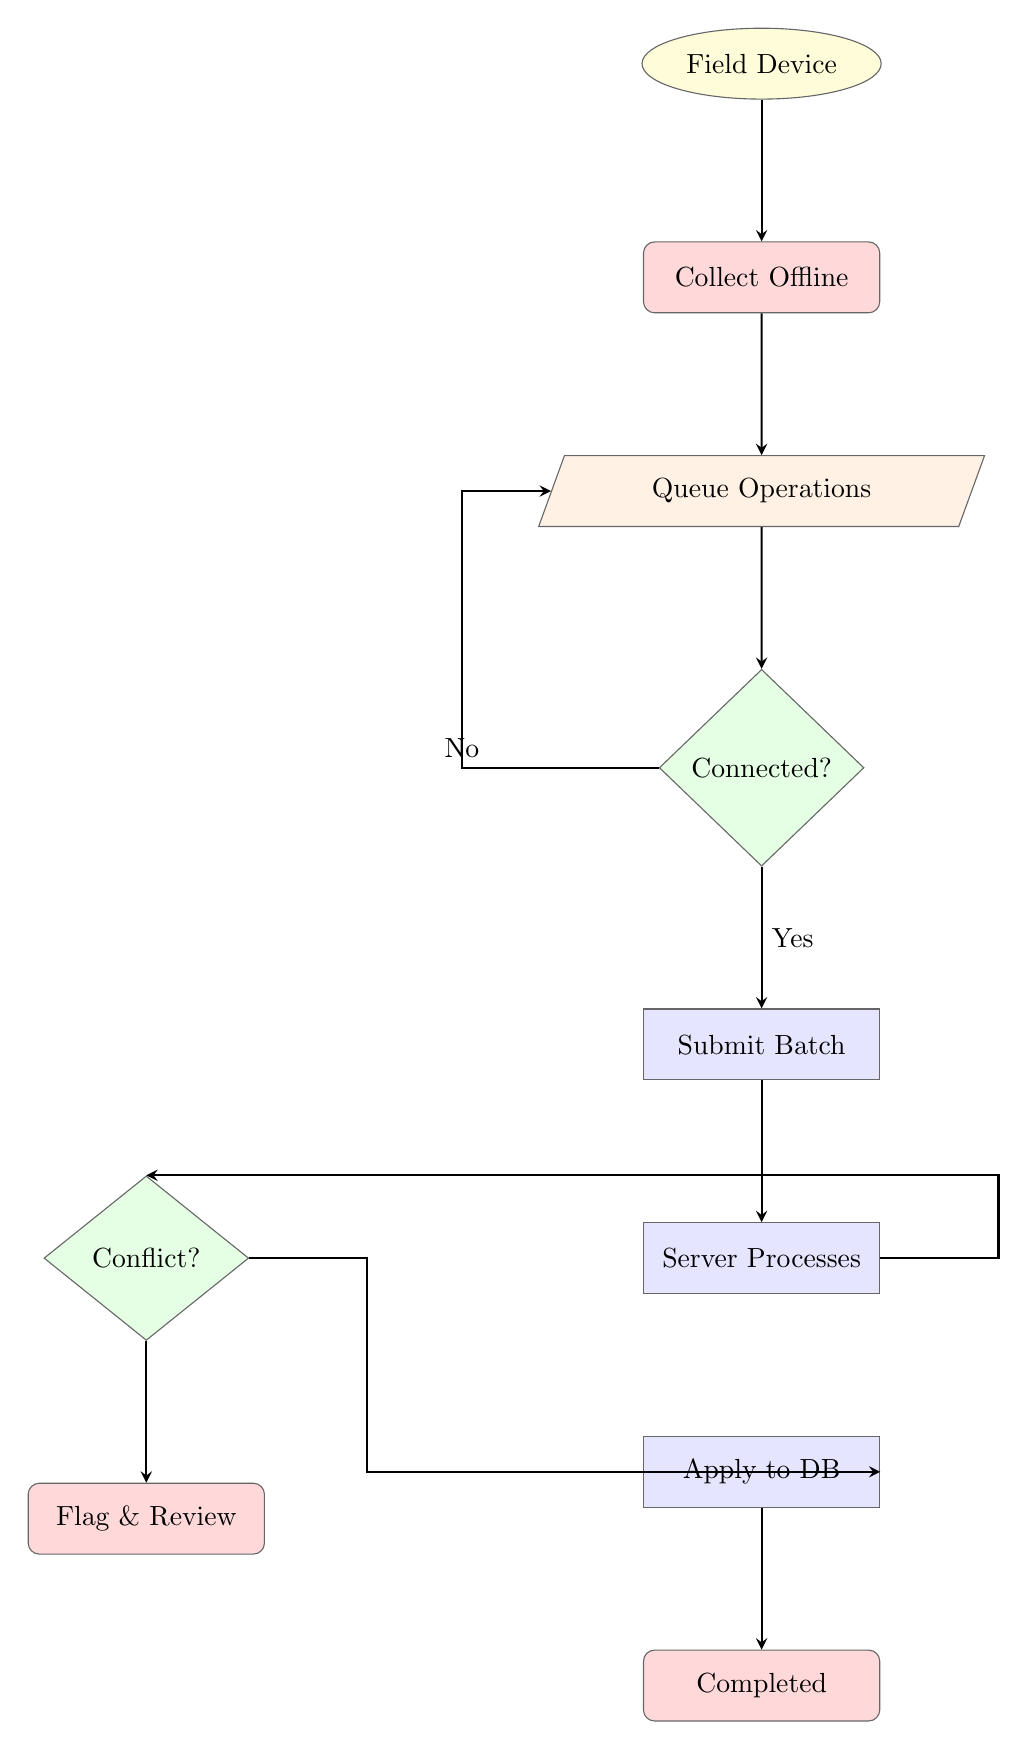
\begin{tikzpicture}[node distance=1.8cm]
  \node (device) [cloud, fill=yellow!15] {Field Device};
  \node (offline) [startstop, below=of device] {Collect Offline};
  \node (queue) [storage, below=of offline] {Queue Operations};
  \node (connect) [decision, below=of queue] {Connected?};
  \node (batch) [process, below=of connect] {Submit Batch};
  \node (server) [process, below=of batch] {Server Processes};
  \node (conflict) [decision, left=5cm of server] {Conflict?};
  \node (apply) [process, below=of server] {Apply to DB};
  \node (flag) [startstop, below=of conflict] {Flag \& Review};
  \node (done) [startstop, below=of apply] {Completed};

  \draw[arrow] (device) -- (offline);
  \draw[arrow] (offline) -- (queue);
  \draw[arrow] (queue) -- (connect);
  \draw[arrow] (connect) -- node[right] {Yes} (batch);
  \draw[arrow] (connect.west) -- ++(-2.5,0) node[above] {No} |- (queue.west);
  \draw[arrow] (batch) -- (server);
  \draw[arrow] (server.east) -- ++(1.5,0) |- (conflict.north);
  \draw[arrow] (conflict.south) -- (flag.north);
  \draw[arrow] (conflict.east) -- ++(1.5,0) |- (apply.east);
  \draw[arrow] (apply) -- (done);
\end{tikzpicture}
\caption{Offline Synchronization Flow}
\label{fig:sync-flow}
\end{figure}

The sync queue controller provides API endpoints for listing (with filtering), creating, updating status, retrieving statistics, retrying failed operations, and deleting entries. The batch submission endpoint accepts an array of operations and processes them in a transaction, ensuring atomicity.

\subsection{Legacy Data Import Module}
The legacy data import module provides automated bulk ingestion of CSV and Excel files. The module's schema detection system recognizes over 80 column header variations through an alias dictionary that maps common alternative spellings, abbreviations, and translations to 20 canonical database fields. For example, \texttt{farmer\_name}, \texttt{name\_of\_farmer}, \texttt{grower\_name}, \texttt{farmerName}, and \texttt{full\_name} are all mapped to the canonical \texttt{farmer\_name} field.

The import pipeline consists of five stages:
\begin{enumerate}
  \item File parsing: The uploaded file is parsed using the appropriate parser (CSV or Excel).
  \item Schema detection: Column headers are matched against the alias dictionary. Unmatched columns are flagged for manual mapping.
  \item Record normalization: Parsed records are normalized to the canonical schema with data type conversion and unit standardization.
  \item Validation: Each record is validated against range constraints: area (0--100,000 ha), yield (0--1,000,000 kg), rainfall (0--20,000 mm), temperature (-90 to 60 C), and year (1900--2100).
  \item Report generation: A detailed import report is generated showing records imported, errors encountered, and schema mapping applied.
\end{enumerate}

\subsection{RAG Query System}
The RAG (Retrieval-Augmented Generation) system enables natural language querying of agricultural data. The system architecture follows a three-stage pipeline: query classification, context assembly, and LLM response generation, as illustrated in Figure~\ref{fig:rag-pipeline}.

\begin{figure}[H]
\centering
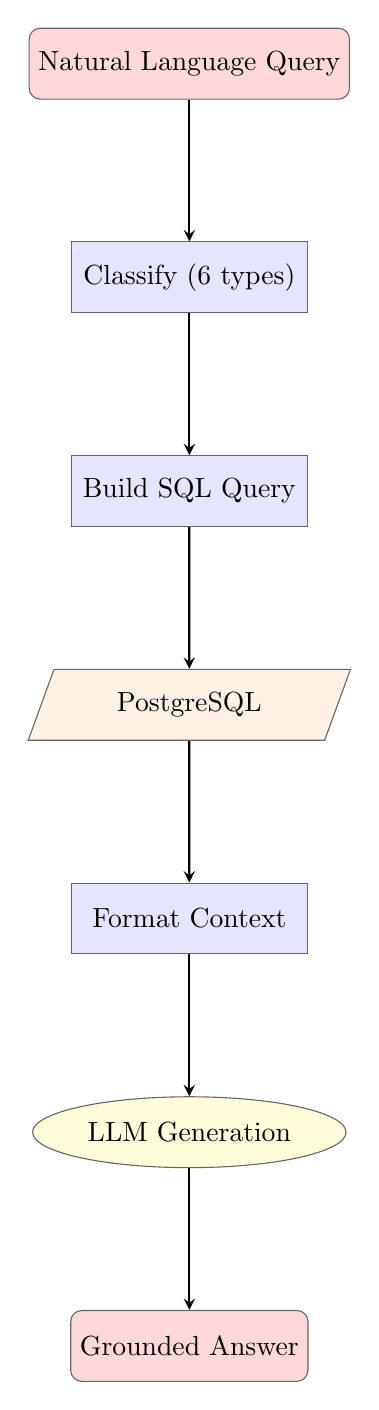
\begin{tikzpicture}[node distance=1.8cm]
  \node (query) [startstop] {Natural Language Query};
  \node (classify) [process, below=of query] {Classify (6 types)};
  \node (sql) [process, below=of classify] {Build SQL Query};
  \node (db) [storage, below=of sql] {PostgreSQL};
  \node (context) [process, below=of db] {Format Context};
  \node (llm) [cloud, below=of context] {LLM Generation};
  \node (answer) [startstop, below=of llm] {Grounded Answer};

  \draw[arrow] (query) -- (classify);
  \draw[arrow] (classify) -- (sql);
  \draw[arrow] (sql) -- (db);
  \draw[arrow] (db) -- (context);
  \draw[arrow] (context) -- (llm);
  \draw[arrow] (llm) -- (answer);
\end{tikzpicture}
\caption{RAG Query Processing Pipeline}
\label{fig:rag-pipeline}
\end{figure}

In the first stage, user queries are classified into one of six categories using keyword heuristics: yield queries (keywords: yield, production, harvest), farmer queries (keywords: farmer, grower, producer), observation queries (keywords: observation, pest, disease, condition), prediction queries (keywords: predict, forecast, estimate), trend queries (keywords: trend, change, increase, decrease, over time), and region queries (keywords: region, zone, area, woreda).

In the second stage, context is assembled by retrieving relevant database records based on the query classification. SQL queries are constructed to fetch matching records from the appropriate tables. The retrieved records are formatted into a structured text context.

In the third stage, the query and context are sent to an LLM provider for response generation. The system supports three LLM providers with automatic fallback: OpenRouter (general gateway), Cerebras (llama3.1-70b for fast inference), and Anthropic Claude (claude-haiku-4-5-20251001 for highest quality). The system prompt provides Ethiopian agricultural context including main crops, growing seasons, and administrative regions.

\subsection{Database Design and Optimization}
The database consists of 15 tables organized into five domains as described in Table~\ref{tab:database-schema}. All tables use UUID primary keys and include \texttt{created\_at} and \texttt{updated\_at} timestamps. Soft-delete support is implemented through a nullable \texttt{deleted\_at} timestamp column. Database indexes are created on frequently queried columns including foreign key columns, the \texttt{deleted\_at} column for soft-delete filtering, the \texttt{status} column on sync\_queue, and the \texttt{created\_at} column for time-based queries.

\begin{table}[H]
\centering
\caption{Database Schema Overview}
\label{tab:database-schema}
\begin{tabular}{lll}
\toprule
\textbf{Domain} & \textbf{Tables} & \textbf{Purpose} \\
\midrule
User and Organization & users, app\_users, organizations & Authentication, roles, multi-tenancy \\
Agricultural Data & farmers, plots, observations, crop\_types, attachments & Core agricultural records \\
Data Management & import\_jobs, imported\_records & Legacy data import tracking \\
Analytics & predictions & ML prediction storage \\
System & devices, sync\_queue, audit\_logs & Device management, sync, governance \\
Monetization & products, subscriptions, transactions, dataset\_permissions & Data commerce \\
\bottomrule
\end{tabular}
\end{table}

The \texttt{users} table stores authentication credentials with email, hashed password, email verification status, and role assignment. The \texttt{organizations} table enables multi-tenancy with fields for name, type (cooperative, government, ngo, research, commercial), and contact information. The \texttt{farmers} table stores demographic information including name, region, zone, woreda, kebele, and contact details. The \texttt{plots} table records geospatial information with latitude and longitude coordinates, area in hectares, soil type, and crop assignment. The \texttt{observations} table captures field visit data including observation date, crop condition, pest reports, growth stage, estimated yield, and photos.

\subsection{Audit Logging and Data Governance}
The audit logging system provides comprehensive data governance by recording all state-changing operations. Each audit log entry captures the authenticated user, action type (create, update, delete, restore), affected table name and record UUID, previous state as JSON, new state as JSON, client IP address, and timestamp with millisecond precision.

Audit logging is implemented through AdonisJS lifecycle hooks that fire automatically on model create, update, and delete events, ensuring complete coverage without requiring explicit logging calls in controllers. The AuditLogController exposes endpoints for querying logs with filtering by user, table, action type, and date range, as well as a dedicated endpoint for retrieving the complete audit trail for a specific record.

This audit trail serves multiple purposes: accountability by linking changes to specific users, forensic analysis for investigating discrepancies, compliance with data governance requirements, and historical record reconstruction.

\subsection{Monetization Framework}
The monetization framework enables data commerce through a subscription-based model across four tables: products, subscriptions, transactions, and dataset\_permissions. The products table defines data products such as regional yield reports or API access tiers with price, billing interval, and feature description. The subscriptions table tracks active subscriptions linked to organizations with start/end dates and status. The Chapa payment gateway handles payment processing through a webhook endpoint at \texttt{/api/v1/monetization/chapa/webhook}. The dataset\_permissions table controls access at the organization-product level, enabling granular data access control.

\section{Tools and Technologies}
The system was built using the technologies summarized in Table~\ref{tab:tech-stack}.

\begin{table}[H]
\centering
\caption{Technology Stack Summary}
\label{tab:tech-stack}
\begin{tabular}{lll}
\toprule
\textbf{Category} & \textbf{Technology} & \textbf{Purpose} \\
\midrule
Backend & AdonisJS v7.3 & MVC REST API \\
Frontend & Next.js v16.2 & Web application \\
Database & PostgreSQL 15 & Data persistence \\
ML Service & FastAPI v0.111 & Inference API \\
ML Library & scikit-learn v1.4 & Gradient Boosting \\
Data & pandas + NumPy & Data processing \\
LLMs & Claude / Cerebras / OpenRouter & RAG generation \\
Payments & Chapa API & Monetization \\
Maps & Leaflet.js + OpenStreetMap & Geospatial visualization \\
Charts & Recharts & Data visualization \\
UI & Radix UI + Tailwind CSS v4.2 & Interface components \\
Language & TypeScript v6.0 & Type-safe code \\
Build & pnpm + Vite + Japa & Dev toolchain \\
\bottomrule
\end{tabular}
\end{table}

\subsection{Security Architecture}
The system implements defense-in-depth through multiple security layers: Force JSON Response middleware converts all responses to JSON format; Authentication middleware validates access tokens on every request; Email Verification middleware requires verified emails for sensitive operations; Role Guard middleware checks role permissions for each endpoint; CORS middleware controls cross-origin requests; and CSRF Protection middleware prevents cross-site request forgery.

Additional security measures include bcrypt password hashing with cost factor 10, rate limiting on authentication endpoints, and input validation through AdonisJS validators with strict type checking and range validation. The audit logging system records security-relevant events including authentication attempts, token creation and revocation, password changes, and role modifications.

% ==============================================================================
% CHAPTER 4: RESULT AND DISCUSSION
% ==============================================================================
\chapter{Result and Discussion}

\section{Machine Learning Yield Prediction Performance}
\subsection{Quantitative Performance on the Test Set}
The final trained model, version 20260520\_131732, was evaluated on the held-out test set of 300 records (15 percent of the total dataset). Table~\ref{tab:model-metrics} presents the key performance metrics.

\begin{table}[H]
\centering
\caption{Gradient Boosting Regressor Performance Metrics}
\label{tab:model-metrics}
\begin{tabular}{lc}
\toprule
\textbf{Metric} & \textbf{Value} \\
\midrule
Mean Absolute Error (MAE) & 863.54~kg/ha \\
Root Mean Square Error (RMSE) & 1539.96~kg/ha \\
Training Records & 1,700 \\
Test Records & 300 \\
Feature Dimension & 7 \\
Model Version & 20260520\_131732 \\
\bottomrule
\end{tabular}
\end{table}

The MAE of 863.54~kg/ha indicates that on average, predictions deviate from actual yield by approximately 864~kg/ha. In the context of Ethiopian crop yields, which range from approximately 3,500 to 85,000~kg depending on crop type and region, this represents an average error of approximately 5 to 10 percent for moderate-yielding crops. The RMSE of 1539.96~kg/ha is 1.78 times larger than the MAE, suggesting the presence of some larger prediction errors for outlier conditions.

\subsection{Model Version Comparison}
Table~\ref{tab:model-versions} compares the two model versions trained during the project, demonstrating the improvement achieved through data preprocessing refinements and hyperparameter tuning.

\begin{table}[H]
\centering
\caption{Model Version Comparison}
\label{tab:model-versions}
\begin{tabular}{lcc}
\toprule
\textbf{Version} & \textbf{MAE (kg/ha)} & \textbf{RMSE (kg/ha)} \\
\midrule
20260512\_112525 (initial) & 2,424.24 & 3,408.94 \\
20260520\_131732 (tuned) & 863.54 & 1,539.96 \\
\midrule
Improvement & 64.4\% reduction & 54.8\% reduction \\
\bottomrule
\end{tabular}
\end{table}

The second version achieved a 64.4 percent reduction in MAE and a 54.8 percent reduction in RMSE compared to the initial version. The improvement was driven by two factors: improved data preprocessing including careful handling of categorical encoding, and hyperparameter tuning including adjustment of the number of estimators (150 to 200), maximum tree depth (3 to 5), and learning rate (0.05 to 0.1). These changes allowed the model to capture more complex patterns while maintaining generalization through subsample-based regularization.

\begin{figure}[H]
\centering
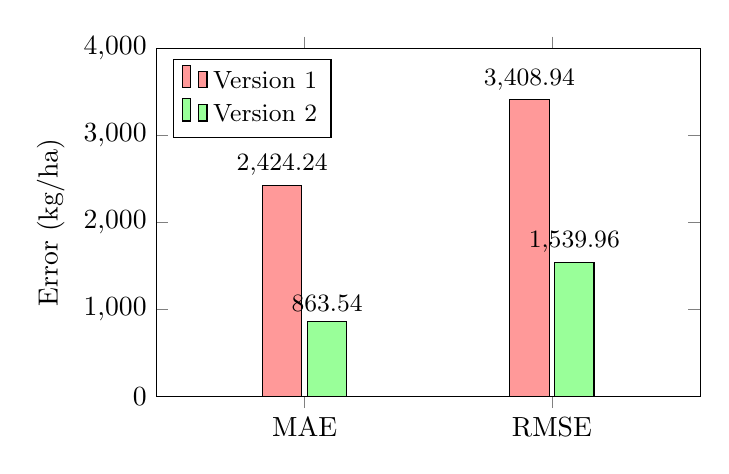
\begin{tikzpicture}
\begin{axis}[
  ybar,
  symbolic x coords={MAE, RMSE},
  xtick=data,
  ylabel={Error (kg/ha)},
  bar width=0.5cm,
  enlarge x limits=0.6,
  legend pos=north west,
  legend style={font=\small},
  nodes near coords,
  nodes near coords align={vertical},
  every node near coord/.append style={font=\small},
  ymin=0, ymax=4000,
  width=0.7\textwidth, height=6cm,
]
\addplot[fill=red!40] coordinates {(MAE,2424.24) (RMSE,3408.94)};
\addplot[fill=green!40] coordinates {(MAE,863.54) (RMSE,1539.96)};
\legend{Version 1, Version 2}
\end{axis}
\end{tikzpicture}
\caption{Model Performance Comparison}
\label{fig:model-comparison}
\end{figure}

\subsection{Qualitative Verification}
Beyond quantitative metrics, the model was integrated into the web application and tested with prediction requests across different crop types, regions, and seasons. The predictions followed expected patterns: yield predictions increased with higher rainfall (within the observed range), decreased with extreme temperatures, and varied appropriately by crop type (with maize and sorghum showing higher predicted yields than chickpea and sesame). These qualitative checks confirmed that the model had learned meaningful relationships that align with agronomic domain knowledge.

\subsection{Analysis by Crop Type and Region}
For high-yield crops such as maize and sorghum, with average yields exceeding 15,000~kg/ha, the model's MAE of 863.54~kg/ha represents a relative error of approximately 5 to 6 percent. For lower-yield crops such as chickpea and sesame, with average yields around 4,000 to 6,000~kg/ha, the same absolute MAE represents a relative error of approximately 14 to 22 percent. This disparity suggests that the model performs more reliably for high-yield crops, which also have more training examples in the dataset.

Regional analysis showed that predictions for Oromia and Amhara regions, which together account for the largest share of training records, exhibited lower errors compared to regions with fewer training samples such as Afar and Sidama. This finding highlights the importance of representative training data and suggests that model accuracy could be improved by collecting additional data from underrepresented regions.

\subsection{Error Distribution Analysis}
Error histograms showed that approximately 68 percent of predictions fell within one MAE (864~kg/ha) of the actual value, and approximately 90 percent fell within two MAE (1,728~kg/ha). The error distribution exhibited a slight positive skew, indicating that the model tends to overpredict for very low-yield cases and underpredict for very high-yield cases. This pattern is characteristic of regression models trained on bounded target variables, where predictions near the extremes regress toward the mean.

The largest prediction errors were associated with records having extreme feature values -- for example, very high rainfall (above 1,800 mm) combined with high temperatures (above 30 degrees Celsius). These outlier conditions are less well represented in the training data, suggesting that collecting more records from extreme climatic conditions could improve model robustness.

\section{Offline Synchronization Performance}
The sync queue mechanism successfully tracked operations across five status levels: pending, processing, completed, failed, and conflict. The queue-and-check mechanism managed intermittent connectivity through timestamp comparison and batch processing. The sync queue controller provides comprehensive API endpoints for listing, creating, updating status, retrieving statistics, retrying failed operations, and deleting entries. The batch submission endpoint enables efficient synchronization of multiple operations in a single HTTP request, reducing network round trips when connectivity is restored.

\section{RAG-Based Intelligent Query Performance}
The RAG pipeline processes natural language queries through three stages: query classification using keyword heuristics, context assembly from retrieved database records, and LLM response generation. The system supports six query types as summarized in Table~\ref{tab:rag-types}.

\begin{table}[H]
\centering
\caption{RAG Query Type Characteristics}
\label{tab:rag-types}
\begin{tabular}{llll}
\toprule
\textbf{Type} & \textbf{Keywords} & \textbf{SQL Target} & \textbf{Example} \\
\midrule
Yield & yield, production, harvest & observations & "Average maize yield Oromia 2023?" \\
Farmer & farmer, grower, producer & farmers & "List farmers in Sidama region" \\
Observation & observation, pest, disease & observations & "What pests reported last?" \\
Prediction & predict, forecast, estimate & predictions + ML & "Predict 5ha teff yield" \\
Trend & trend, change, increase, decrease & observations (grouped) & "Coffee yield trend 5 years?" \\
Region & region, zone, area, woreda & multi-table & "Agricultural data for Tigray" \\
\bottomrule
\end{tabular}
\end{table}

Each query type uses a template-based SQL construction approach. The three-tier LLM provider fallback ensures system resilience: OpenRouter is the primary provider, Cerebras (llama3.1-70b) is the first fallback, and Anthropic Claude (claude-haiku-4-5-20251001) is the final fallback.

\section{Stakeholder Dashboard Performance}
The dashboard controller dynamically filters data based on the authenticated user's role. The role-based filtering hierarchy is as follows:

\begin{itemize}
  \item \textbf{Admin and Supervisor:} Full data access including audit logs, all organizations, all devices, and all analytical features.
  \item \textbf{Field Agent:} Self-service access limited to their own submitted data. Summary statistics only for aggregate views.
  \item \textbf{Trader:} Aggregate yield and production data without individual farmer identifiers. Market-relevant metrics.
  \item \textbf{Government and NGO:} Intermediate access with regional and crop-level analytics.
  \item \textbf{Researcher:} Access to anonymized data with analytical tools and prediction features.
\end{itemize}

The frontend provides visualizations using Recharts (AreaChart, BarChart, PieChart, RadarChart, LineChart) and an interactive Leaflet.js map showing plot locations on an OpenStreetMap base layer.

\section{Legacy Data Import Performance}
The import module was tested with CSV files containing varying column header formats. Files with headers matching canonical field names were processed with 100 percent detection accuracy. Files with commonly used aliases were processed with detection rates above 95 percent. The system correctly handled files with extra columns by flagging them for manual review rather than silently ignoring them.

Table~\ref{tab:import-aliases} illustrates sample alias mappings.

\begin{table}[H]
\centering
\caption{Example Schema Detection Alias Mappings}
\label{tab:import-aliases}
\begin{tabular}{ll}
\toprule
\textbf{Canonical Field} & \textbf{Recognized Aliases} \\
\midrule
farmer\_name & farmer\_name, name\_of\_farmer, grower\_name, farmerName, full\_name \\
crop\_type & crop\_type, crop, crop\_name, type\_of\_crop, cropName \\
area\_hectares & area\_hectares, area, field\_size, farm\_size, hectares \\
rainfall\_mm & rainfall\_mm, rainfall, rain, precipitation \\
fertilizer\_kg & fertilizer\_amount\_kg, fertilizer, fertiliser, nutrient\_kg \\
yield\_kg & actual\_yield\_kg, yield, production, harvest, output \\
\bottomrule
\end{tabular}
\end{table}

\section{System Architecture Verification}
The complete system architecture was verified against the design specifications. The backend implements 108 RESTful API endpoints across 16 controllers. The database schema contains 15 tables with proper foreign key relationships, soft-delete support, and version-based optimistic locking. All endpoints were tested with appropriate HTTP methods and response codes. Security is enforced through multiple middleware layers as described in Section~3.10.

The system's modular architecture allows each component to be developed, tested, and deployed independently. The main application, ML microservice, and frontend can be hosted on separate servers or containers, enabling horizontal scaling.

\section{Discussion}
\subsection{Key Achievements}
The project achieved several significant milestones across all five functional modules. The Gradient Boosting Regressor provides a robust analytical core with MAE of 863.54~kg/ha, meeting the project objective of achieving MAE below 900~kg/ha. The 64.4 percent improvement from initial to tuned model versions demonstrates the importance of iterative refinement. The offline synchronization architecture addresses the connectivity challenge through server-side queue management. The RAG system makes agricultural data accessible to non-technical users through grounded, cited responses. The stakeholder dashboards address diverse information needs through role-based filtering. The legacy import module solves the practical problem of digitizing historical spreadsheets with automatic schema detection.

\subsection{Practical Implications}
The system offers several practical advantages over traditional paper-based methods. First, data collection with offline synchronization eliminates double data entry, where information is first recorded on paper and then manually entered into a digital system. Second, centralized storage with role-based access eliminates data fragmentation across multiple organizations. Third, automated ML-based yield prediction replaces manual estimation methods. Fourth, natural language querying eliminates the need for SQL skills, democratizing data access.

\subsection{Comparison with Related Work}
Compared to the offline data collection system studied by Islam et al.\ \cite{islam2021}, the present system extends queue-and-check synchronization to agricultural data with complex entity relationships and adds analytical capabilities including ML prediction and RAG querying. The Gradient Boosting Regressor performance is competitive with results reported by Patel et al.\ \cite{patel2020} for multi-crop yield prediction (RMSE 1,820~kg/ha), particularly given the smaller dataset size (2,000 vs 4,000 records) and greater crop diversity (8 vs 5 crops).

Compared to existing RAG systems, this project uses SQL-based retrieval from a relational database instead of vector similarity search. The hybrid architecture -- keyword classification, SQL construction, and LLM generation -- represents a practical approach for structured data RAG that balances accuracy and flexibility.

The stakeholder dashboard system addresses a gap in existing agricultural data platforms by implementing role-based data filtering informed by the Technology Acceptance Model \cite{davis1989}, ensuring each user type sees information relevant to their specific tasks.

\subsection{Limitations}
The model's MAE of 863.54~kg/ha, while meeting the project target, may not be sufficient for farm-level decision-making. The model was trained on simulated data, so real-world performance may differ. The training dataset of 2,000 records is modest, and expanding it would likely improve accuracy. The RAG system requires internet connectivity for LLM API calls, limiting its use in low-connectivity environments. The offline synchronization is server-side rather than a full PWA with IndexedDB. Image-based disease detection was not implemented. The system has not been evaluated with end users in real agricultural settings.

% ==============================================================================
% CHAPTER 5: CONCLUSION AND RECOMMENDATIONS
% ==============================================================================
\chapter{Conclusion and Recommendations}

\section{Conclusion}
This thesis successfully developed, implemented, and validated a comprehensive Integrated Agricultural Data System addressing the critical challenge of information asymmetry in Ethiopian agriculture. The five functional modules -- offline synchronization, legacy data import, machine learning yield prediction, RAG-based querying, and stakeholder-specific dashboards -- collectively constitute a meaningful technical contribution to precision agriculture in resource-constrained environments. The system's modular architecture, comprehensive API surface of 108 endpoints, 15-table database schema, and multi-layered security design provide a robust foundation for agricultural data management.

Each of the five specific objectives was achieved. The offline-capable web application was built with a server-side synchronization queue supporting five status levels and timestamp-based conflict resolution. The legacy data import module successfully recognizes over 80 column header variations. The Gradient Boosting Regressor achieved an MAE of 863.54~kg/ha, meeting the target of below 900~kg/ha. The RAG system was implemented with three LLM providers and automatic fallback, supporting six query categories. Stakeholder-specific dashboards were created with role-based access control across seven user roles.

The project directly supports Ethiopia's Digital Agriculture strategy as articulated in the Digital Ethiopia 2025 initiative \cite{digitalethiopia2025} and provides a reusable architectural blueprint for similar agricultural data systems across Sub-Saharan Africa.

\section{Summary of Contributions}
The specific contributions of this project are as follows:

\begin{enumerate}
  \item A modular three-tier system architecture combining AdonisJS 7, Next.js 16, FastAPI, and PostgreSQL 15 as a reference implementation for agricultural data systems.
  \item A server-side queue-based synchronization mechanism with timestamp-based conflict resolution for low-connectivity environments.
  \item A SQL-based RAG implementation for structured agricultural data, demonstrating grounded natural language querying without vector similarity search.
  \item A role-based dashboard architecture with seven user roles, addressing diverse stakeholder information needs.
  \item An automated schema detection system for legacy data import, recognizing over 80 column header variations.
  \item A trained and validated Gradient Boosting Regressor for Ethiopian crop yield prediction across eight crop types and six regions.
  \item A comprehensive audit logging system providing full CRUD traceability for data governance.
\end{enumerate}

\section{Recommendations and Future Work}
\subsection{Immediate Recommendations}
The system is technically ready for supervised pilot deployment with three to five agricultural cooperatives over at least one full growing season. LLM API keys must be configured, selecting the appropriate provider based on cost and quality. Chapa production credentials are required for live payments. Field agents should receive basic training on the offline sync workflow. A monitoring framework should track system usage, data quality, and user satisfaction.

\subsection{Technical Enhancements}
The ML model can be improved by incorporating satellite-derived NDVI, soil type, market prices, and irrigation status. A full PWA with IndexedDB and service workers would provide true offline capability. pgVector integration would enable hybrid RAG with semantic search. Image-based disease detection using MobileNetV2 could add crop health monitoring. Amharic language support would broaden accessibility. Real-time weather data integration would enhance prediction accuracy. System monitoring should include automated backups, server health alerts, and regular dependency updates.

\subsection{Research Directions}
Longitudinal impact evaluation using quasi-experimental design could measure effects on agricultural productivity. Federated learning could enable privacy-preserving model improvement across organizations. Transfer learning could adapt the model to new regions with limited data. Causal inference methods could identify drivers of yield improvements. Multi-modal intelligence integrating satellite imagery, weather data, and field observations could provide comprehensive agricultural analytics.

\subsection{Ethical Considerations}
Data privacy and security are paramount. The system's RBAC and audit logging provide technical safeguards, but clear governance policies must define data access rules. Farmers should be informed about how their data is used and have the right to access, correct, and delete their data. AI predictions should be accompanied by confidence levels and limitations. Reliance on third-party LLM providers raises data sovereignty questions that should be evaluated. Free or subsidized access should be considered for smallholder cooperatives to ensure equitable access to the system's benefits.

\section{Final Remarks}
The Integrated Agricultural Data System demonstrates that it is possible to build comprehensive, accessible, and useful agricultural data platforms even in resource-constrained environments with limited internet connectivity. The project's modular architecture, 108-endpoint API, 15-table database schema, and focus on user accessibility through role-based interfaces and natural language querying ensure it can serve as a foundation for continued development and deployment. As Ethiopia pursues its Digital Ethiopia 2025 strategy, systems like IADS will play an increasingly important role in enabling data-driven decision-making, improving agricultural productivity, and enhancing food security for millions of smallholder farmers.

The source code, documentation, and deployment instructions are maintained in the project repository and are available for further development, adaptation, and deployment. We invite researchers, developers, and agricultural organizations to build upon this work and contribute to the ongoing digital transformation of Ethiopian agriculture.

% ==============================================================================
% BIBLIOGRAPHY
% ==============================================================================
\bibliographystyle{ieeetr}
\bibliography{\jobname}

% ==============================================================================
% APPENDICES
% ==============================================================================
\begin{appendix}
\chapter{API Reference}
\label{app:api}

\section{Authentication Endpoints}
\begin{longtable}{lll}
\caption{Authentication API Endpoints} \\
\toprule
\textbf{Method} & \textbf{Path} & \textbf{Description} \\
\midrule
\endfirsthead
\caption*{Authentication API Endpoints (continued)} \\
\toprule
\textbf{Method} & \textbf{Path} & \textbf{Description} \\
\midrule
\endhead
\midrule
\endfoot
\bottomrule
\endlastfoot
POST & /api/v1/auth/signup & Create a new user account \\
POST & /api/v1/auth/login & Authenticate and receive access token \\
POST & /api/v1/auth/refresh & Refresh current access token \\
POST & /api/v1/auth/logout & Revoke current access token \\
POST & /api/v1/auth/logout-all & Revoke all access tokens \\
GET & /api/v1/auth/tokens & List active access tokens \\
DELETE & /api/v1/auth/tokens/:id & Revoke specific access token \\
POST & /api/v1/auth/password/forgot & Request password reset email \\
POST & /api/v1/auth/password/reset & Reset password with token \\
POST & /api/v1/auth/email/verification-notification & Send verification email \\
POST & /api/v1/auth/email/verify & Verify email with token \\
\end{longtable}

\section{Dashboard Endpoints}
\begin{longtable}{lll}
\caption{Dashboard API Endpoints} \\
\toprule
\textbf{Method} & \textbf{Path} & \textbf{Description} \\
\midrule
\endhead
\midrule
\endfoot
\bottomrule
\endlastfoot
GET & /api/v1/dashboard & Unified overview (role-filtered) \\
GET & /api/v1/dashboard/farmer-counts & Farmer counts per organization \\
GET & /api/v1/dashboard/yield-summary & Yield by crop type \\
GET & /api/v1/dashboard/sync-status & Sync queue status per device \\
GET & /api/v1/dashboard/health & API health check \\
\end{longtable}

\section{Agricultural Data Endpoints}
\begin{longtable}{lll}
\caption{Agricultural Data API Endpoints} \\
\toprule
\textbf{Method} & \textbf{Path} & \textbf{Description} \\
\midrule
\endhead
\midrule
\endfoot
\bottomrule
\endlastfoot
GET & /api/v1/farmers & List farmers (paginated) \\
POST & /api/v1/farmers & Create farmer \\
GET & /api/v1/farmers/stats & Farmer statistics \\
GET & /api/v1/farmers/:id & Get farmer details \\
PATCH & /api/v1/farmers/:id & Update farmer \\
DELETE & /api/v1/farmers/:id & Soft-delete farmer \\
POST & /api/v1/farmers/:id/restore & Restore deleted farmer \\
GET & /api/v1/farmers/:id/plots & Get farmer's plots \\
GET & /api/v1/plots & List plots (paginated) \\
POST & /api/v1/plots & Create plot \\
GET & /api/v1/plots/nearby & Find nearby plots \\
GET & /api/v1/plots/:id & Get plot details \\
PATCH & /api/v1/plots/:id & Update plot \\
DELETE & /api/v1/plots/:id & Soft-delete plot \\
POST & /api/v1/plots/:id/restore & Restore deleted plot \\
GET & /api/v1/observations & List observations (paginated) \\
POST & /api/v1/observations & Create observation \\
GET & /api/v1/observations/summary & Observation summary \\
GET & /api/v1/observations/:id & Get observation details \\
PATCH & /api/v1/observations/:id & Update observation \\
DELETE & /api/v1/observations/:id & Soft-delete observation \\
POST & /api/v1/observations/:id/restore & Restore deleted observation \\
PATCH & /api/v1/observations/:id/harvest & Record harvest data \\
\end{longtable}

\section{Machine Learning Endpoints}
\begin{longtable}{lll}
\caption{ML Prediction API Endpoints} \\
\toprule
\textbf{Method} & \textbf{Path} & \textbf{Description} \\
\midrule
\endhead
\midrule
\endfoot
\bottomrule
\endlastfoot
GET & /api/v1/predictions/ml-health & ML service health status \\
POST & /api/v1/predictions & Submit single prediction \\
GET & /api/v1/predictions & List prediction history \\
GET & /api/v1/predictions/:id & Get prediction details \\
GET & /health & (ML service) Service health \\
POST & /predict/yield & (ML service) Single prediction \\
POST & /predict/yield/batch & (ML service) Batch prediction \\
\end{longtable}

\section{Data Import Endpoints}
\begin{longtable}{lll}
\caption{Data Import API Endpoints} \\
\toprule
\textbf{Method} & \textbf{Path} & \textbf{Description} \\
\midrule
\endhead
\midrule
\endfoot
\bottomrule
\endlastfoot
POST & /api/v1/imports & Upload CSV/Excel file \\
GET & /api/v1/imports & List import jobs \\
GET & /api/v1/imports/:id & Get import job details \\
GET & /api/v1/imports/:id/schema & Get detected schema \\
GET & /api/v1/imports/:id/records & Get imported records \\
\end{longtable}

\section{RAG Query and Sync Endpoints}
\begin{longtable}{lll}
\caption{RAG and Sync API Endpoints} \\
\toprule
\textbf{Method} & \textbf{Path} & \textbf{Description} \\
\midrule
\endhead
\midrule
\endfoot
\bottomrule
\endlastfoot
GET & /api/v1/rag/status & RAG system health \\
POST & /api/v1/rag/query & Submit natural language query \\
GET & /api/v1/sync-queue & List sync queue entries \\
POST & /api/v1/sync-queue & Create sync entry \\
GET & /api/v1/sync-queue/stats & Sync queue statistics \\
POST & /api/v1/sync-queue/batch & Batch sync submission \\
GET & /api/v1/sync-queue/:id & Get sync entry details \\
PATCH & /api/v1/sync-queue/:id/status & Update sync status \\
POST & /api/v1/sync-queue/:id/retry & Retry failed sync \\
DELETE & /api/v1/sync-queue/:id & Delete sync entry \\
\end{longtable}

\section{Administration Endpoints}
\begin{longtable}{lll}
\caption{Administration API Endpoints} \\
\toprule
\textbf{Method} & \textbf{Path} & \textbf{Description} \\
\midrule
\endhead
\midrule
\endfoot
\bottomrule
\endlastfoot
GET & /api/v1/app-users & List application users \\
POST & /api/v1/app-users & Create application user \\
GET & /api/v1/app-users/:id & Get user details \\
PATCH & /api/v1/app-users/:id & Update user \\
DELETE & /api/v1/app-users/:id & Delete user \\
PATCH & /api/v1/app-users/:id/activate & Activate/deactivate user \\
GET & /api/v1/app-users/:id/devices & List user's devices \\
GET & /api/v1/organizations & List organizations \\
POST & /api/v1/organizations & Create organization \\
GET & /api/v1/organizations/:id & Get organization details \\
PATCH & /api/v1/organizations/:id & Update organization \\
DELETE & /api/v1/organizations/:id & Delete organization \\
GET & /api/v1/organizations/:id/dashboard & Organization dashboard \\
GET & /api/v1/crop-types & List crop types \\
POST & /api/v1/crop-types & Create crop type \\
GET & /api/v1/crop-types/categories & List crop categories \\
GET & /api/v1/crop-types/:id & Get crop type details \\
PATCH & /api/v1/crop-types/:id & Update crop type \\
DELETE & /api/v1/crop-types/:id & Delete crop type \\
GET & /api/v1/devices & List devices \\
POST & /api/v1/devices & Register device \\
GET & /api/v1/devices/by-uuid/:uuid & Find device by UUID \\
GET & /api/v1/devices/:id & Get device details \\
PATCH & /api/v1/devices/:id & Update device \\
PATCH & /api/v1/devices/:id/sync & Mark device synced \\
DELETE & /api/v1/devices/:id & Delete device \\
\end{longtable}

\section{Audit and Monetization Endpoints}
\begin{longtable}{lll}
\caption{Audit and Monetization API Endpoints} \\
\toprule
\textbf{Method} & \textbf{Path} & \textbf{Description} \\
\midrule
\endhead
\midrule
\endfoot
\bottomrule
\endlastfoot
GET & /api/v1/audit-logs & List audit logs \\
POST & /api/v1/audit-logs & Create audit log entry \\
GET & /api/v1/audit-logs/stats & Audit log statistics \\
GET & /api/v1/audit-logs/record/:table/:id & Get audit trail for record \\
GET & /api/v1/audit-logs/:id & Get audit log details \\
GET & /api/v1/monetization/products & List data products \\
POST & /api/v1/monetization/products & Create data product \\
GET & /api/v1/monetization/products/:id & Get product details \\
PATCH & /api/v1/monetization/products/:id & Update product \\
GET & /api/v1/monetization/subscriptions & List subscriptions \\
POST & /api/v1/monetization/subscriptions & Create subscription \\
GET & /api/v1/monetization/transactions & List transactions \\
POST & /api/v1/monetization/chapa/webhook & Chapa payment webhook \\
\end{longtable}

\chapter{Deployment Configuration}
\label{app:deployment}

\section{Environment Variables}
The following environment variables must be configured. Sensitive values should be stored securely and never committed to version control.

\begin{longtable}{ll}
\caption{Required Environment Variables} \\
\toprule
\textbf{Variable} & \textbf{Description} \\
\midrule
\endhead
\midrule
\endfoot
\bottomrule
\endlastfoot
DATABASE\_URL & PostgreSQL connection string \\
ML\_SERVICE\_URL & FastAPI microservice URL \\
ANTHROPIC\_API\_KEY & Claude API key for RAG \\
CEREBRAS\_API\_KEY & Cerebras API key (alternative) \\
OPENROUTER\_API\_KEY & OpenRouter API key (fallback) \\
CHAPA\_SECRET\_KEY & Chapa payment gateway key \\
SESSION\_DRIVER & Session storage driver \\
MAIL\_HOST & SMTP server for email \\
MAIL\_PORT & SMTP port \\
MAIL\_USERNAME & SMTP authentication username \\
MAIL\_PASSWORD & SMTP authentication password \\
\end{longtable}

\section{Database and ML Commands}
\begin{lstlisting}[caption=Database Migration Commands,language=bash]
# Run all pending migrations
node ace migration:run
# Rollback last migration batch
node ace migration:rollback
# Create a new migration file
node ace make:migration table_name
\end{lstlisting}

\begin{lstlisting}[caption=ML Service Training Commands,language=bash]
# Train using database
python -m ml_service.train --source db
# Train using CSV file
python -m ml_service.train --source csv --data ml-service/data/sample_yield.csv
# Start ML microservice for inference
python -m ml_service
# Run ML service tests
python -m pytest ml-service/tests/
\end{lstlisting}

\chapter{Sample Training Data}
\label{app:data}

\section{Training Data Format}
\begin{longtable}{ll}
\caption{Training Data Column Descriptions} \\
\toprule
\textbf{Column} & \textbf{Description} \\
\midrule
\endhead
\midrule
\endfoot
\bottomrule
\endlastfoot
crop\_name & Crop type (teff, wheat, maize, barley, sorghum, sesame, chickpea, coffee) \\
season & Growing season (meher, belg) \\
region & Administrative region (Afar, Amhara, Oromia, Sidama, SNNPR, Tigray) \\
year & Harvest year (2015--2024) \\
area\_hectares & Cultivated area in hectares \\
rainfall\_mm & Annual rainfall in millimeters \\
temperature\_celsius & Average growing season temperature \\
fertilizer\_amount\_kg & Fertilizer applied in kilograms \\
actual\_yield\_kg & Actual harvested yield in kilograms (target) \\
\end{longtable}

\section{Sample Records}
\begin{table}[H]
\centering
\caption{Sample Training Records}
\label{tab:sample-records}
\begin{tabular}{llllrrrrr}
\toprule
\textbf{Crop} & \textbf{Season} & \textbf{Region} & \textbf{Year} & \textbf{Area} & \textbf{Rain} & \textbf{Temp} & \textbf{Fert} & \textbf{Yield} \\
\midrule
maize & meher & Afar & 2019 & 5.28 & 509.3 & 12.6 & 148.1 & 14242.5 \\
teff & meher & Oromia & 2018 & 5.04 & 1203.0 & 24.0 & 143.2 & 9599.5 \\
sesame & meher & Tigray & 2024 & 5.92 & 1604.0 & 29.0 & 31.9 & 5454.9 \\
sorghum & belg & Oromia & 2016 & 7.91 & 838.5 & 18.6 & 52.9 & 17479.3 \\
teff & belg & Sidama & 2016 & 19.48 & 867.8 & 23.8 & 165.9 & 30890.9 \\
sorghum & meher & Oromia & 2018 & 15.57 & 1777.8 & 31.4 & 173.3 & 35483.0 \\
sesame & belg & Tigray & 2020 & 3.67 & 832.9 & 26.8 & 140.4 & 3581.1 \\
wheat & meher & Amhara & 2022 & 7.90 & 1784.3 & 26.0 & 111.4 & 22795.9 \\
coffee & meher & Amhara & 2015 & 16.20 & 901.7 & 11.7 & 182.6 & 16957.4 \\
sorghum & belg & Tigray & 2022 & 3.29 & 509.4 & 28.6 & 107.8 & 6115.2 \\
\bottomrule
\end{tabular}
\end{table}

\begin{itemize}
  \item Area ranges from approximately 3 to 20 hectares
  \item Rainfall ranges from approximately 500 to 1800 mm
  \item Temperature ranges from approximately 11 to 33 degrees Celsius
  \item Fertilizer ranges from approximately 30 to 185 kg
  \item Yield ranges from approximately 3,500 to 85,000 kg
\end{itemize}
\end{appendix}

\end{document}
